\chapter{Град Киев на Лысой}

Теперь вернемся на перекресток улицы Кирилловской-Фрунзе с Нижнеюрковской и отправимся по Кирилловской в сторону Кирилловской церкви. Так проще будет говорить о местности и открытиях, тут сделанных.

По правую руку – безликая промзона на равнине Оболонья, или, как говорили в конце 19, начала 20 веков – Плоской части. Слева же, поначалу в некотором отдалении, вызванном деятельностью человека – цепь холмов, слывущих Кирилловскими высотами.

С давних пор вдоль них было множество кирпичных и пивных заводов, в которых надо четко разбираться, дабы «читать» упоминания об археологических находках, где привязка идет обычно следующая – «в усадьбе такого-то завода». Путь наш разобьем на участки. Первый – по улице Кирилловской, между пересекающимися с нею улицей Нижнеюрковской и Мыльным переулком. Всё, что нас интересует, расположено на нечетной, левой по нашему ходу, стороне Кирилловской.

Сначала идет неработающий кирпичный завод по адресу Нижнеюрковская, 2. Участок принадлежит ОАО «Керамблоки». Огороженный с двух сторон завод расположен на углу Кирилловской и Нижнеюрковской, на последней и проходная. Попасть на территорию можно лишь обходным путем, по склонам. Напрямую не пустят.

А ведь там, за стеной и корпусами, самое важное. Частично я уже ранее рассказал об этой, ныне срытой, бывшей юго-восточной части Лысой горы. Точно на территории бывших заводов кирпичного и солодовых экстрактов, между улицей Кирилловской и склоном горы – плоская местность, которую я часто и неверно именую «нижнее плато». На аэрофотоснимке 1943 года там еще заметна возвышенность. Перед окончательным ее уничтожением, летом 1965 года археологи под руководством Е. В. Максимова провели там раскопки, о которых в печати можно узнать по скудному набору печатных источников, самый объемный из которых – статья «Могильник X века на горе Юрковице» самого Максимова совместно с Р. С. Орловым из 41-го номера украинского журнала «Археология» за 1982 год.

\begin{center}
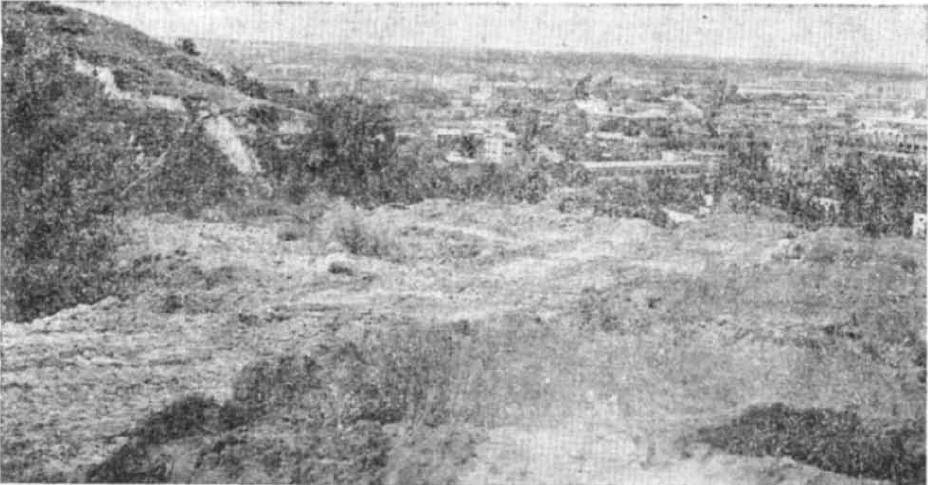
\includegraphics[width=\linewidth]{chast-kirvys/lys02/maxfoto.jpg}

\textit{1965. Вид с юга на место раскопок.}
\end{center}

В экспедиции принимали участие сам Максимов, а также Анна Шовкопляс, П. Толочко, А. Кубышев, Б. Брязкун. Юрковицей Максимов называл только юго-восточ\-ный отрог, пожираемый кирпичным заводом, всю же гору именовал Лысой. На 1965 год от этой Юрковицы сохранился лишь останец длиной 60 и шириной 40 метров, с ровной наверху площадкой, немного наклоненной на север и разделенной на две части большой вымоиной, восточной и западной.

Я не могу понять, о какой именно местности идет речь, несмотря на приложенный к статье план, составленный С. Д. Крыжицким, и плохого качества фотоснимок.

\begin{center}
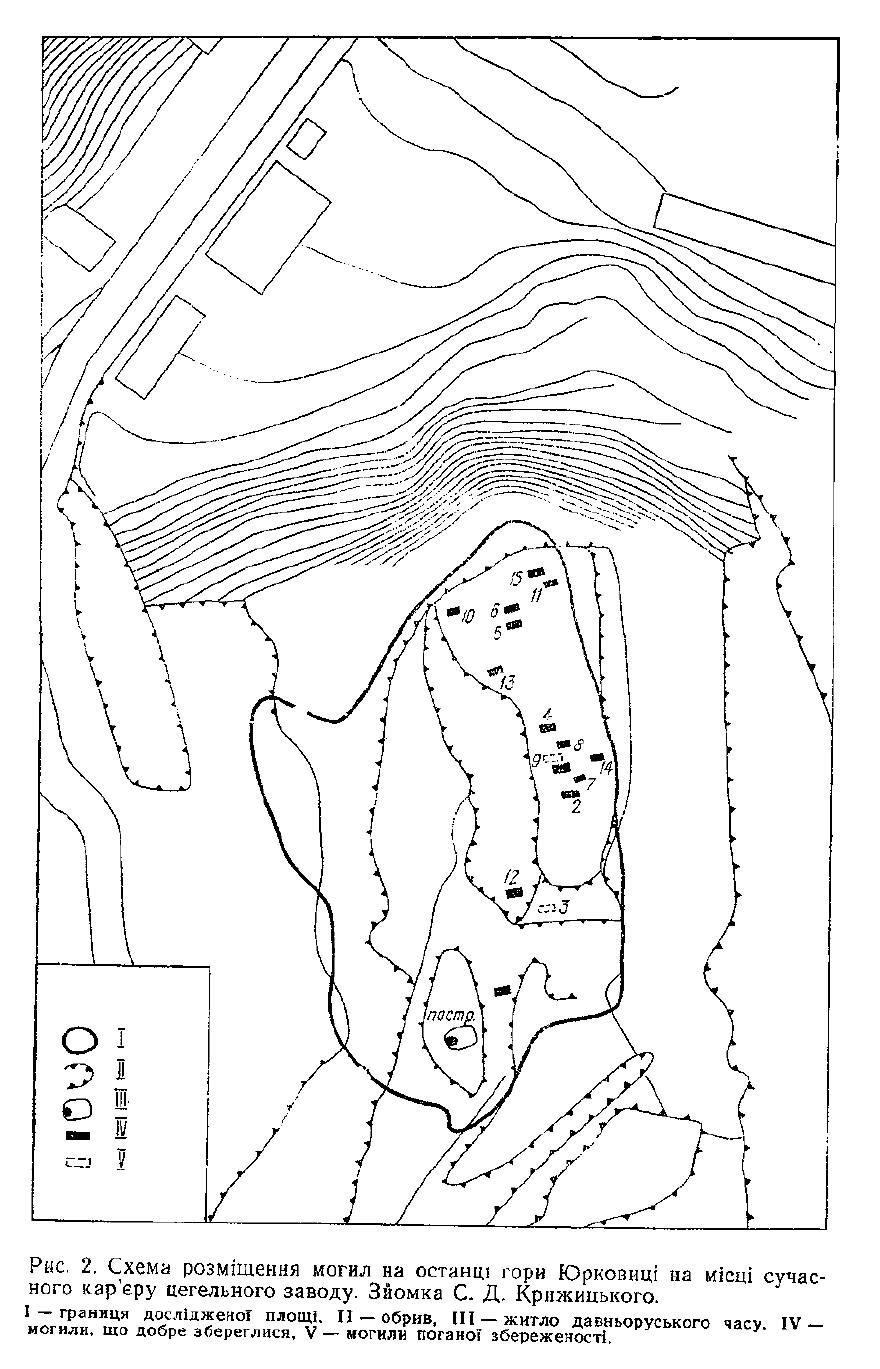
\includegraphics[width=0.92\linewidth]{chast-kirvys/lys02/maxplan2.jpg}
\end{center}

Зачем составлять план, где не обозначена  ориентация, а также не подписаны улицы? Он бесполезен для читателя – тогда для чего помещать его в статье?

Что это за прямая улица сверху слева? Кирилловская или Нижнеюрковская? Если на другой ее стороне – тоже холм, значит последняя, но мои попытки наложить карту на современную с учетом этого провалились. Вымоина же, делящая останец с севера на юг, и упоминание, что на месте пригорка теперь (в 1982 году) – карьер – позволяет предположить, что раскопки велись там, где нынче «плато» южнее Кирилловской 49, но это лишь моя догадка.

В северо-восточной части «Юрковицы» археологи нашли «остатки поселения чернолесского типа VIII – первой половины VII века до нашей эры». На восточной части склона, по краю, был черноземный вал, перекрывавший ямы и жилье, датируемое указанными веками, сам же вал археологи соотнесли с культурным слоем «поселения зарубинецкой культуры, которое находилось на северо-восточном краю горы и датируется концом II-I столетий до нашей эры». Статья сообщает:

\begin{quotation}
Около западного склона в давнем подъярке длиной 40 м, шириной 8-11 м и глубиной 6 м [...] найдено значительное количество обломков посуды чернолесского и зарубинецкого типов, а также фрагменты эллинистичных амфор, железных ножей, наконечник стрелы, фибулу и прочее.
\end{quotation}

Основная часть статьи посвящена 16-ти могилам на горе, связываемых учеными к христианским погребениям и «древнерусскому времени» (10 веку), хотя каких-либо указаний на эти выводы я не вижу.

Скелеты лежали в гробах, на спине, головой к западу. Среди них нашли различные предметы – железные гвозди, кольца, замок с дужкой, ножи, были также мелочи вроде бронзовых пуговиц, кольцо из медной проволоки, гирька весом примерно в 4 грамма, да обломки деревянного, с обручами ведра. 

Неподалеку от могил, на юго-западном краю останца, было какое-то строение, углами ориентированное по сторонам света, небольшое (3,90х2,70 м), с печкой. В нем же обломки горшков, изготовленных на гончарном круге, им археологи дают 10 век нашей эры. Кстати, ориентировка зданий по сторонам света была присуща Подолу до пожара 1811 года.

Почти никак, помимо кратких упоминаний, не отражены раскопки 1965 года на Юрковице-новой в книге Максимова 1982 года «Зарубинецкая культура на территории СССР», дважды по половине страницы уделены этим раскопкам в книге Максимова же, 1972 года, «Среднее Поднепровье на рубеже нашей эры». Выпишу оттуда. Мое стремление свести воедино сведения об этом месте обусловлены представлением, что на Лысой горе был город Кия, поэтому всё, связанное с этим, крайне важно.

\begin{quotation}
Поселение открыто В. Д. Дяденко. [...] Культурный слой поселения был перемещен в овраг, проходивший близ западного склона горы. Это было сделано в конце XIX ст. при создании кирпичного завода, когда верхние слои снимались до слоя керамической глины. Лишь на окраине останца удалось открыть два очага и пять хозяйственных ям зарубинецкого времени. 

В овраге найдено около 5000 фрагментов зарубинецкой керамики. Кухонные горшки изготовлялись из глины, содержащей примесь песка. Поверхность ровная, шершавая, коричневого цвета, форма и орнамент обычные (ямки, выдавленные пальцем, или косые насечки). Днища плоские, без закраины. Диаметр днищ до 10 см, отверстия горшка по венчику 16-25 см. Некоторые стенки имели хроповатую поверхность. 

Найдены обломки корчаг и плоские диски-сковородки. Встречены шершавые миски скифоидного типа с прямым или загнутым внутрь краем. Чернолощеная керамика представлена горшками, мисками, кружками с ручкой. Преобладают острореберные экземпляры. Лощение высокого качества. 

Встретились фрагменты стенок античных амфор, по определению И. Б. Зеест, эллинистического времени, пряслиц, куски железных шлаков, стенка горна\footnote{Тут руду перерабатывали в крицу. Важнейшая находка перечисляется второстепенно.}, обломки железных ножей с горбатой спинкой, наконечник копья с коротким острием круглые в сечении шилья. 

Найдены бронзолитейный тигель\footnote{И снова!}, проволочная фибула среднелатенской конструкции, пластинчатый браслет, спиральное кольцо, стержень, бронзовый трехгранный наконечник стрелы с внутренней втулкой III в. до н. э., гранитные терочники и пастовая зеленая бусина с глазками.
\end{quotation}

В другом месте книги Максимов пишет:

\begin{quotation}
На восточной оконечности этого останца был отмечен невысокий (0,9 м) вал шириной 3,8 м, проходивший по самому краю поселения. За ним начинался искусственный крутой (до 50 градусов) склон (эскарп) длиной 6 м, оканчивавшийся неширокой (1,2 м) горизонтальной площадкой, за которой уже шел естественный, более пологий, склон холма.

При разрезе вала было установлено, что он состоял из черноземного грунта, взятого с примыкающей к валу площадки поселения. В нем встретились немногочисленные обломки керамики предскифского (чернолесского) периода, относимого к VIII в. до н. э., происходящие из культурного слоя поселения этого времени, остатки которого были открыты нами в восточной части горы.

Эти данные свидетельствуют о том, что вал на Юрковице был насыпан не в чернолесское время, а позднее – в зарубинецкую эпоху или же в период Киевской Руси. Однако Киевская Русь как время сооружения вала на этом поселении исключается, поскольку здесь тогда существовал могильник, погребения которого были исследованы Н. Ф. Беляшевским и нами.
%Укрепления Юрковицы были построены в зарубинецкое время, вероятно, в I в. до н. э., о чем свидетельствует найденный на поселении, вблизи вала, фрагмент гладкой проволочной среднелатенской фибулы.
\end{quotation}

Однако насколько верно Максимов отождествляет место своих раскопок с местом раскопок Беляшевского? Сколь верны датировки?

Относительно заселенности Лысой горы во время Киевской Руси в науке существует странное предубеждение. Дескать, жили только по Подол включительно, а всё, что откопали севернее, вдоль Кирилловских высот – это надо датировать каким угодно временем, только не «Киевской Русью». Исключение составляют, конечно же, могилы. Мол, хоронить могли и при «Киевской Руси».

%Я не знаю, как лучше, чтобы всё устроилось. Валы эти частью уже уничтожены разным строительством. Но внимание науки также приводит к уничтожению памяти прошлого, точнее, к переработке. Нарушается покой чужого праха, останки извлекаются из могил, курганы срываются. Почему давние кладбища можно разорять? Я понимаю раскопки какого-нибудь мусора, красиво именуемого «культурным слоем» – на деле это не более чем мусор, а мусор в любое время отражает культуру не только текущую, но и прошлую. Если я ношу часы 1951 года выпуска, и потерял их в 2020, это не значит, что место, где я их посеял, относится к 1951-му. Да еще попробуйте датируйте часы без старого каталога от производителя! А насколько точны датировки глиняных горшков? Но примем в целом, что слой мусора отражает проявления некоторого времени. 

%Рытье котлована при строительстве здания или прокладке коллектора либо метро – случайно задели что-то древнее, археологи приходят, изучают. Есть возможность, понимаю! Но когда знают заранее, что собираются проводить «раскопки» на древнем кладбище – не принимаю. Сколько времени должно пройти со времени похорон человека, чтобы археология считала себя вправе разрыть его могилу? Пара сотен лет? Да нет, это еще считается вандализмом. Ну а, допустим, пятьсот лет? Моооожно!

%Однако, нравы таковы, что не доберутся «белые» археологи, так займутся «черные», только вместо оседания ценностей в запасниках музеев находки пойдут на продажу, а кости – кому до них есть дело?

\begin{center}
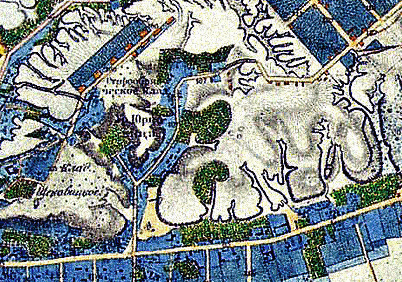
\includegraphics[width=\linewidth]{chast-kirvys/lys02/1865.png}

\textit{Фрагмент карты 1865 года. «Рогатка» Нижнеюрковской в форме Y, полный (не сожранный карьерами) юго-восточный склон – справа от нижней палочки Y. Улица внизу поперек всего – Кирилловская.}
\end{center}

Кроме изученного в 1965 году вала, всего в нескольких сотнях метрах от него, науку долго ждали другие валы – на соседних отрогах к северу и югу. Некоторые из них известны ей давно, с 19 века. До некоторых уже не успеть дойти пешком – снесены либо застроены.

%Меня всё еще удивляет, что Киев – такой город, где летописное и более далекое прошлое находится на расстоянии пешей прогулки. Не надо ехать за тридевять земель, знай себе ходи по городу с широко открытыми глазами. Но предпочитали ехать в Херсонес и Ольвию, в то время как древние урочища Киева зарастали не лесом, а непроходимыми массивами гаражей.

Археологи снова занялись раскопками на территории кирпичного завода, предварительными, только в 2014 году, и обнаружили «древнерусский культурный слой».

Кирпичный завод возник очень давно и за несколько веков сожрал б\'ольшую часть того, что могло остаться от летописного «града Киева», сооруженного братьями Кием, Хоривом и Щеком. Зловредное дело уничтожения древних залежей началось по крайней мере с 18 века.

А вот неразбериха, которую я распутывать не буду, однако приведу условия задачи. На плане 1752 года, на углу современных улиц Кирилловской и Нижнеюрковской, показаны кирпичные заводы Ивана Григоровича (Барского), «который речку Юрковицу прибрал на одну сажень». Почти у самой Рогатки, с середины 18 века, работал и кирпичный завод Кирилловского монастыря. С 1765 года\footnote{После секуляризации церковных земель манифестом 1764 года Екатерины II, отнявшим у церкви большинство её землевладений.} некий завод здесь же перешел в руки влиятельной дворянской семьи Гудимов-Левковичей. И Григорович, и Гудимы были в 18 веке время арендаторами земель у Кирилловского монастыря.

На середину 19 века завод Левковичей стал, наряду с эйсмановским, одним из крупнейших частных кирпичных заводов. Тогда докопались до залегавшей на уровне Днепра синей глины, из которой получался отличный желтоватый кирпич, ставшей визитной карточкой строений в Киеве того времени. Во второй половине 19 века, ближе к восьмидесятым, количество кирпичных заводов на Кирилловских высотах, Сырце, околицах Вышгорода и южнее Киева стремительно росло, старые заводы с глинищами (карьерами) перекупались, производство расширялось.

В 1894 году Михаил Вильгельмович Рихерт приобрел заводы кирпичный и смежный с ним пивоваренный Псиола, что стоял на углу перекрестка Юрковской и Кирилловской. По другим данным, кирпичный был взят в аренду у Екатерины Гудим-Левкович.

\begin{center}
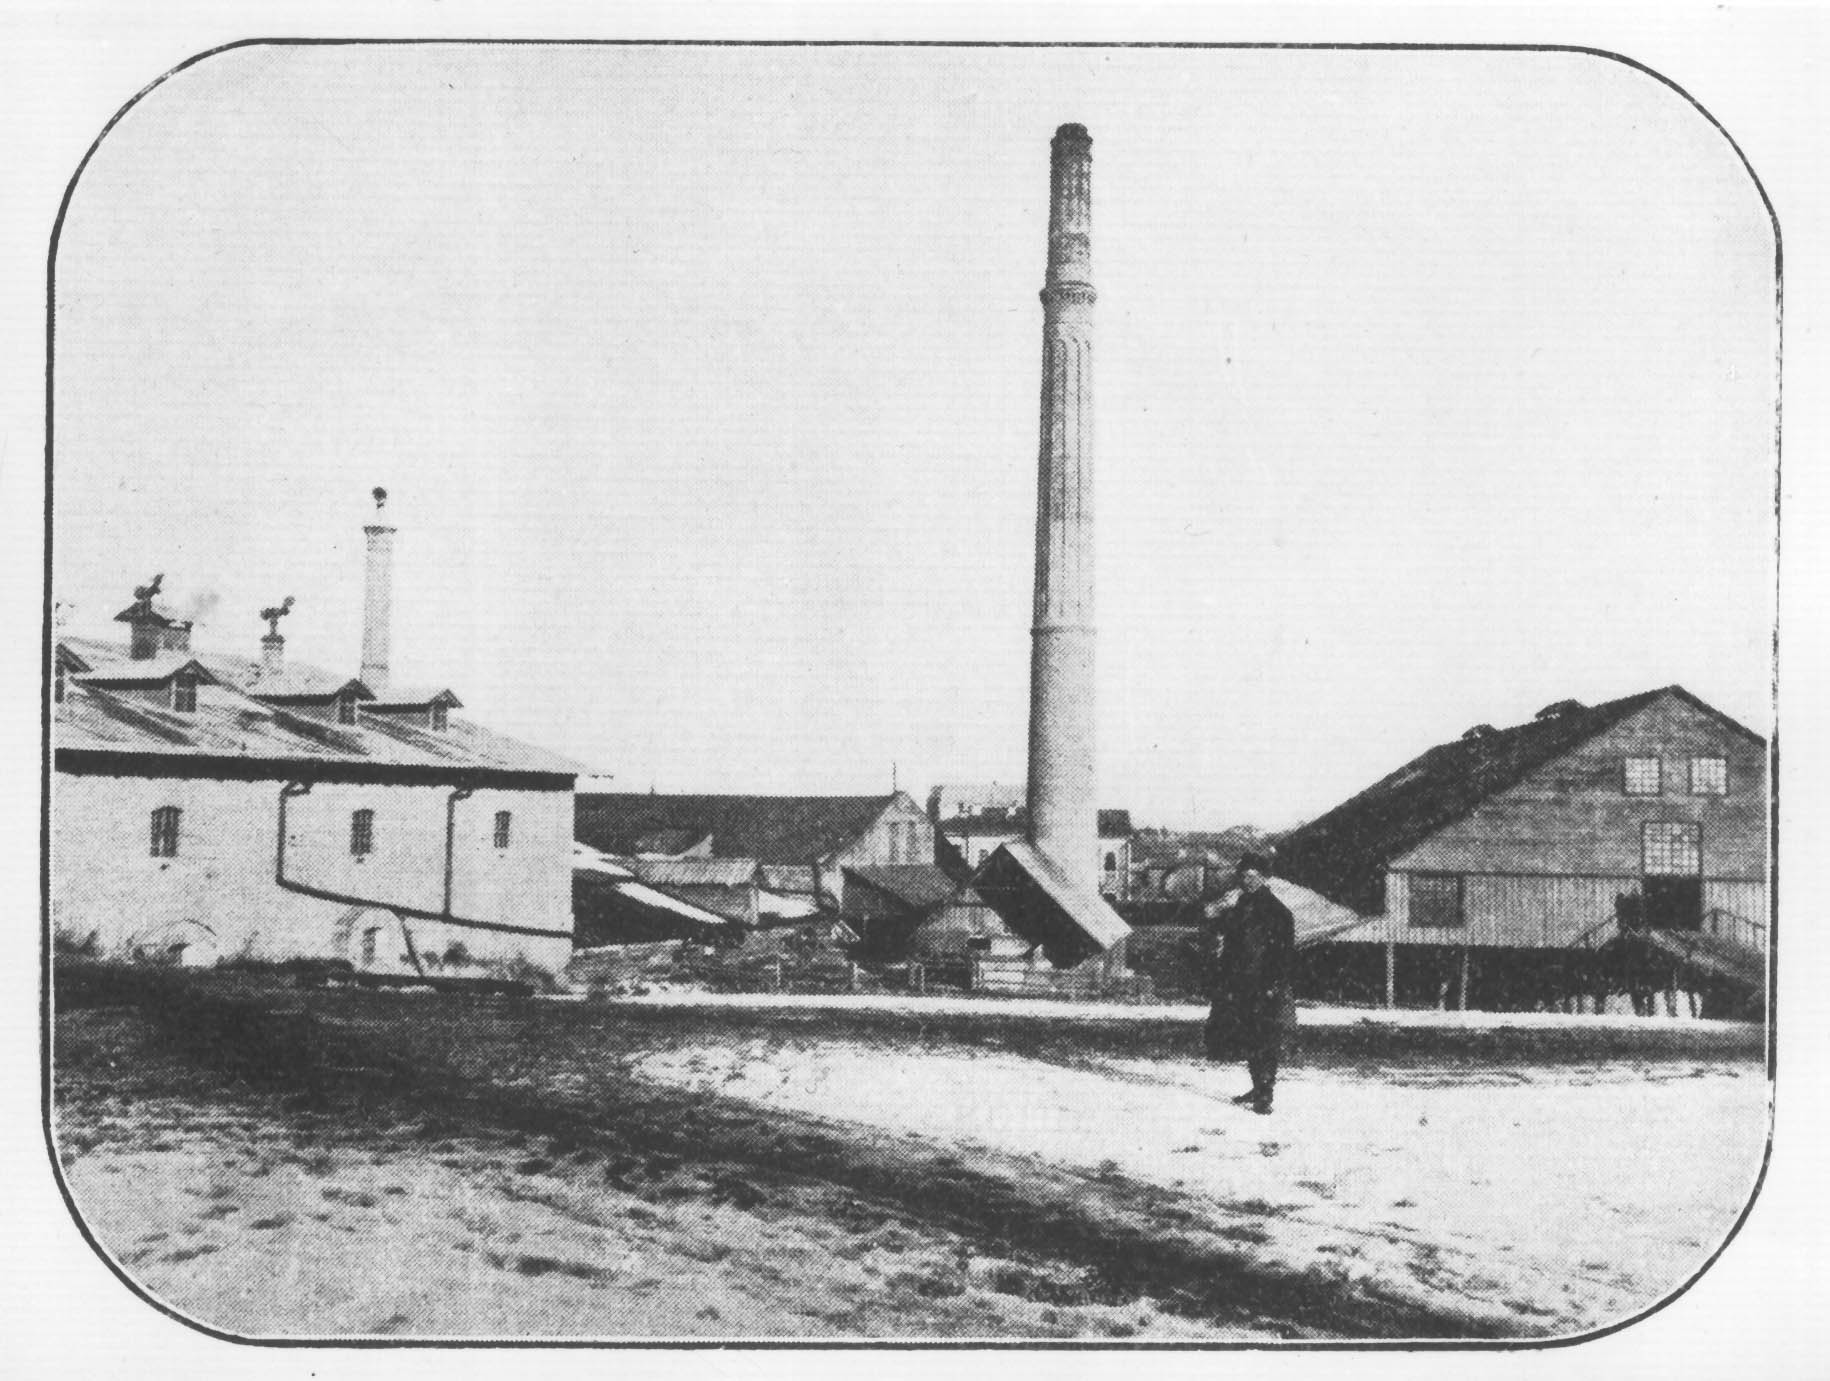
\includegraphics[width=\linewidth]{chast-kirvys/lys02/1897-rihert-kirp.jpg}

\textit{Усадьба кирпичного и пивного заводов Рихерта в 1897 году. Труба в центре находится сейчас позади здания по адресу Кирилловская 35.}
\end{center}

До начала строительных работ на участке завода, либо во время оно, там раскопали курган с женским языческим погребением, датированным второй половиной 10 века. Доклад о находке сделал барон де Бай, не то сам проводивший раскопки, не то купивший находки оттуда. Извлеченное из могилы барон увез в Париж – две бронзовые вызолоченные застежки в форме черепахи, две серебряные серьги, ожерелье из бус сердоликовых, горного хрусталя, серебра, янтаря; крестообразную подвеску к ожерелью – на подвеске были византийские монеты, чеканенные между 928 и 944 годами, с именами василевсов Романа I, Константина X, Стефана. Позже де Бай передал всё это российской Археологической комиссии, и теперь предметы находятся в Московском историческом музее.

Но вернемся к истории завода. Рихерт поставил всё на широкую ногу. В 1895 году возвел каменную печь системы Гофмана, для обжига кирпича-сырца, с высокой трубой под самое небо – это её видно на снимке. Годовой оборот – 20000 рублей.

Годы Первой мировой, революция, гражданка. В одном из витков вихрей войн и революций кирпичный завод Рихерта наползает на соседний кирпичный завод баронессы Фиркс, до революции имевший адрес Нижнеюрковской 4 и 6 – окрестности нынешней воинской части.

Банкротство завода Рихерта. Последующее восстановление пленными немцами и венграми. Создание на его основе предприятия «Керамблоки», перепрофилирование на выпуск канализационных труб – это 1932 год. В 1948 году налаживается выпуск облицовочной плитки. После Великой Отечественной войны в усадьбе завода были общежития для рабочих, клуб с патефоном и, позже, телевизором. Рабочие находили время для театральной самодеятельности. Барак, где жили рабочие, имел адрес Нижнеюрковская, 4 и стоял на пригорке над тогдашним карьером.

К 1950-м доля кирпича увеличилась до 85 процентов. Продолжался выпуск плитки разных видов, в том числе мозаичной глазированной. 1978 год – кирпичные блоки для детских садов. Восьмидесятые – спад производства.

В 1894 году Михаил Рихерт купил, рядом с кирпичным заводом, пиво-медоваренный завод Псиола (Псело). На 2014 год, это недействующий завод Солодовых экстрактов, по адресу Кирилловская, 35. 

Пивзавод здесь, еще в 1860 году, построил отставной штабс-капитан С. Псело, после смерти коего в 1867 году завод перешел к его племяннице, А. Псело. У отца Михаила Рихерта, Вильгельма, на Куренёвке, по современному адресу Сырецкая, 19, работал мощнейший пивоваренный завод. Теперь это Киевский завод шампанских вин «Столичный». У Вильгельма было два брата, Яков и Михаил. Сырецким заводом, по смерти отца, сначала владели оба, а потом Якову остался завод на Сырце, а Михаил приобрел этот вот рядом с кирпичным.

Тоже – переоборудование. В 1908 году архитектор Николай Казанский построил главный корпус, похожий на английский замок. После революции завод неоднократно менял профиль – выпускал безалкогольные напитки, патоку для карамели, а с 1956 года солодовые экстракты – приготовленные из проросших злаков сиропы, использующиеся в пищевой промышленности. В 2006 году завод сей, с 1993 года принадлежащий ООО «Киевский завод солодовых экстрактов», закрылся, успев впрочем напечатать рекламный календарь. К тому времени предприятие производило не только экстракты, но и концентраты кваса, лимонады, и многое другое. Десять лет прошло, осенью 2013 году основное здание подрихтовали и выставили на продажу. 

\begin{center}
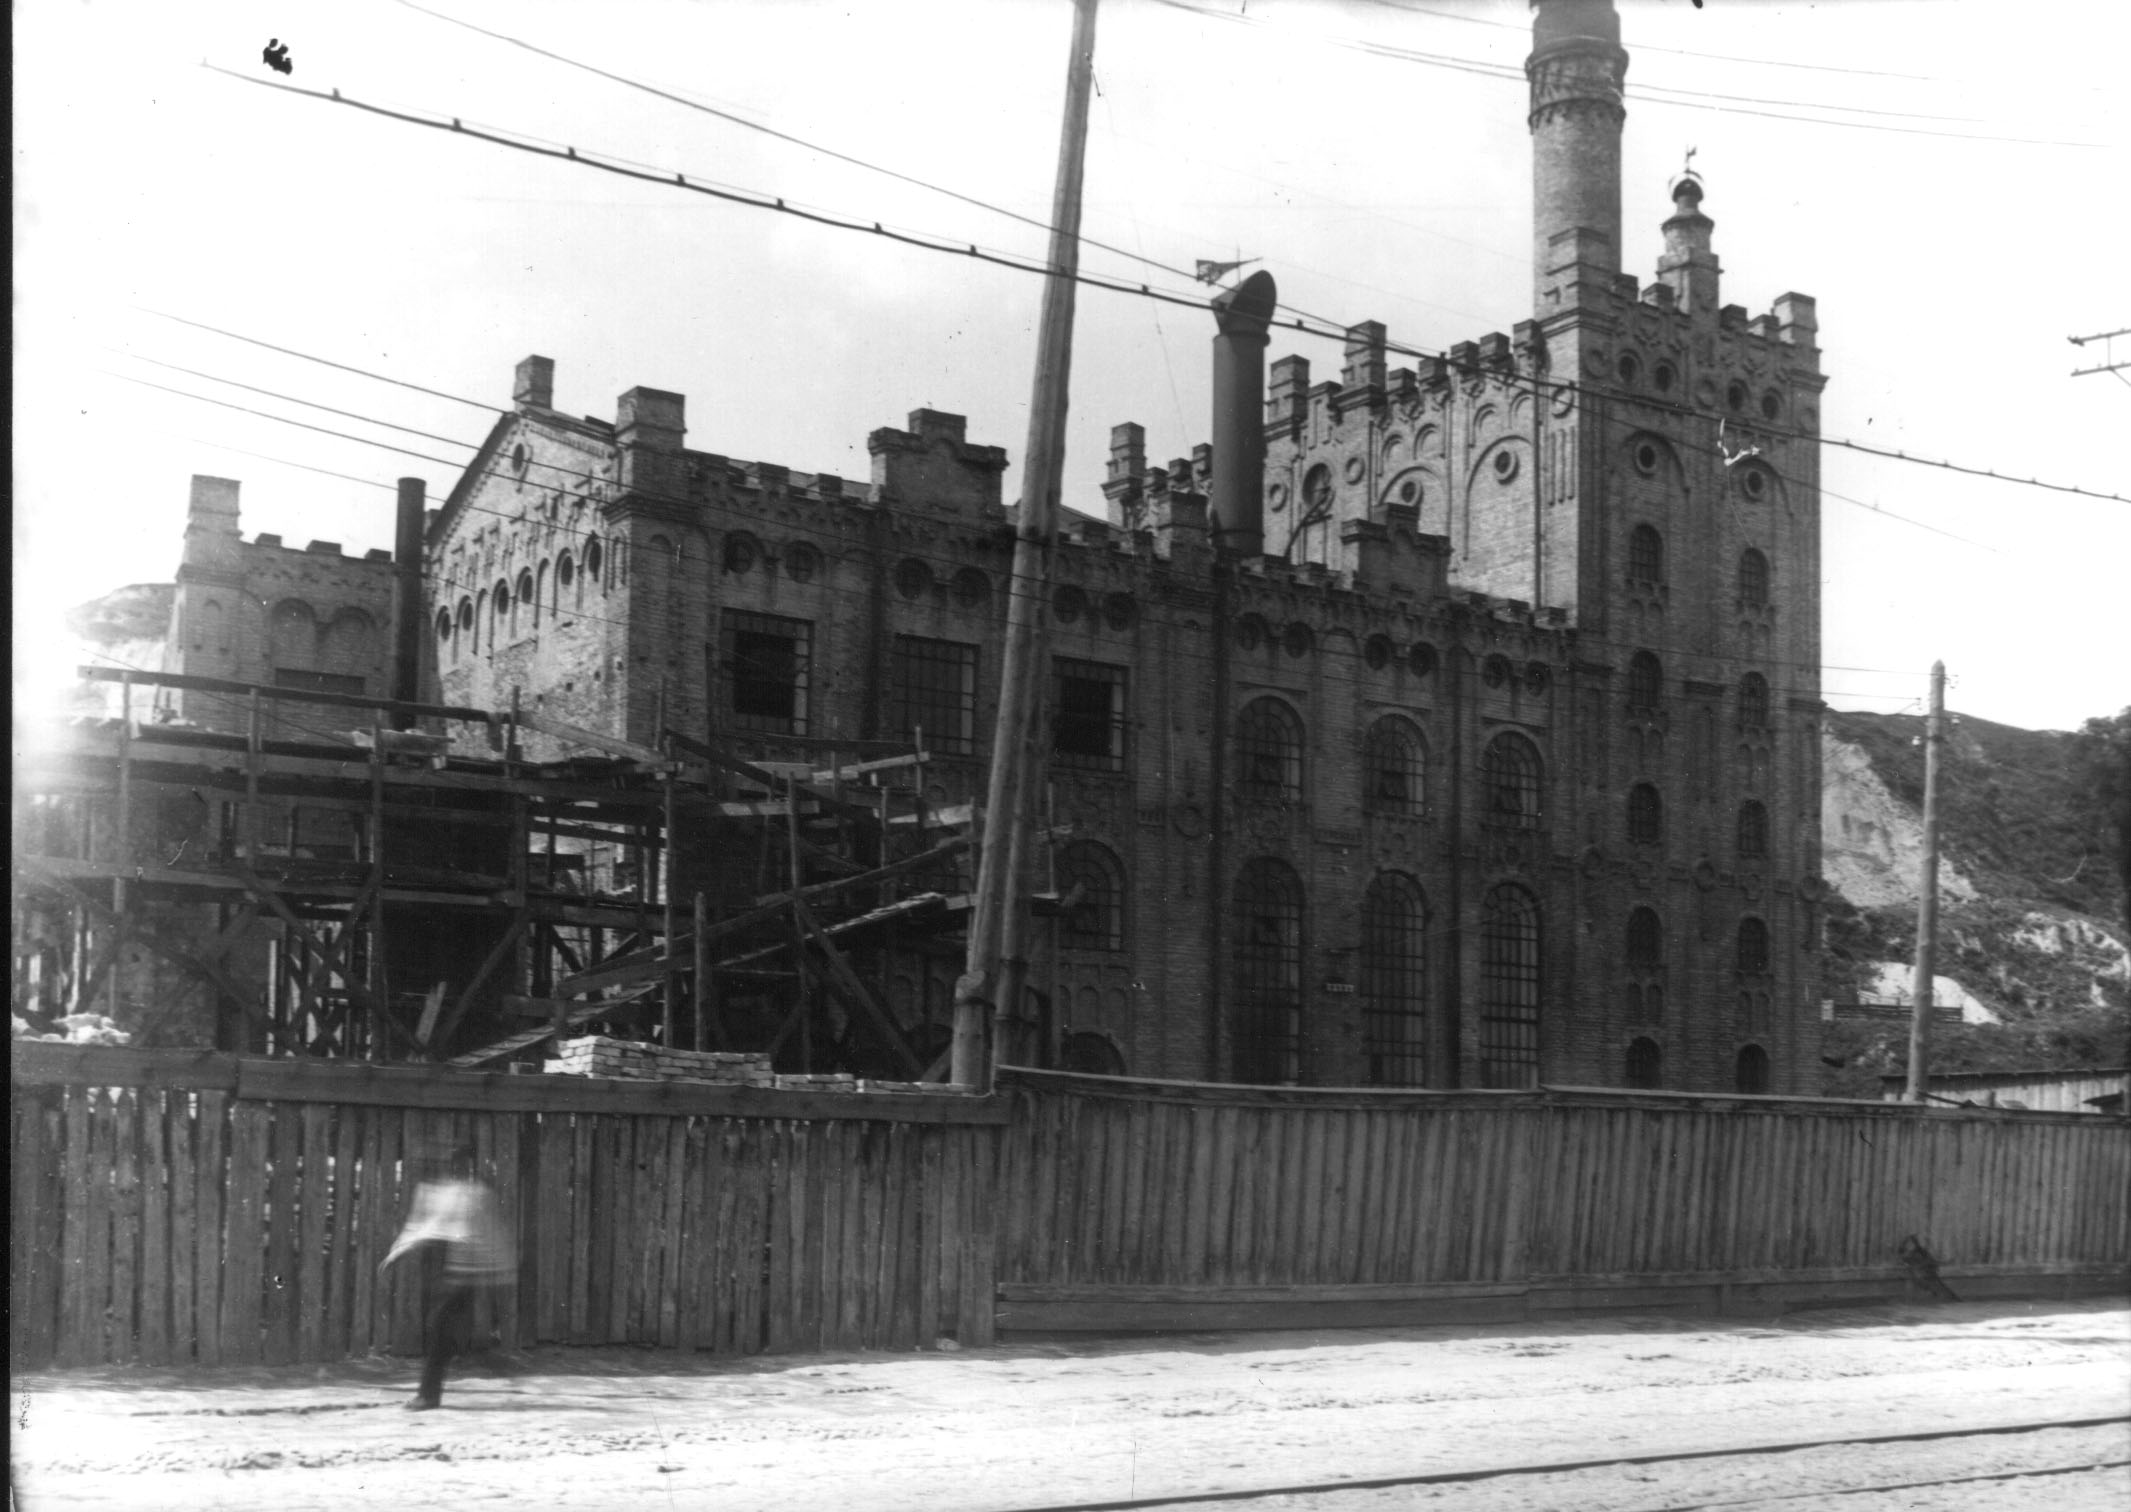
\includegraphics[width=\linewidth]{chast-kirvys/lys02/1940-riherta.jpg}

\textit{Пивзавод Рихерта в 1940-е, справа видна срытая позже часть склона Лысой горы.}
\end{center}

Двигаемся по улице Кирилловской дальше, но всё не доходим до Мыльного переулка. Еще один пивзавод, действовавший до 2014 года. Адрес – Кирилловская 41, «ЗАО Пивзавод на Подоле». Это бывший завод «Общества Киевского пивоваренного завода», дореволюционные адреса корпусов коего были, в разное время, на Кирилловской 41-47.

История такова. С некоторых времен, там стоял кирпичный завод, где вроде бы в 1821 году случился пожар, перебросившийся к соседней Иорданской Николаевской церкви и спаливший её дотла. Уцелел ли тогда кирпичный завод, неведомо, однако в 1835 году купец Петр Никитич Дехтерёв купил там у мещанки Татьяны Ботвинской усадьбу (2700 кв. сажней, за 5415 рублей серебром) и обустроил там чугунолитейный завод, перешедший в 1853-1864 годах к сыну купца, Родиону. К 1871 году это крупное предприятие, производящее оборудование для сахарной и винокуренной промышленности, пришло в упадок, и было куплено вместе с участком купцом первой гильдии Николаем Григорьевичем Хряковым.

Хряков – предприимчивый сын крестьянина Льговского уезда Харьковской губернии, в 1861 году переселился в Киев и развел здесь бурную деятельность – продавил создание Киевской биржи (здание на углу Институтской и Крещатика было разрушено немцами во время Великой Отечественной войны), способствовал строительству Политеха в 1890-е, попутно с общественно-полезной деятельностью наращивал обороты – стал сахарозаводчиком, работал в банковой сфере, состоял гласным (депутатом) городской думы. Втихаря перечислял бедным семействам вспоможения. Жил в доме №17 на Большой Подвальной, умер в начале мая 1900 года, похоронен был на кладбище у Аскольдовой могилы.

И вот Хряков с компаньонами Карлом Вейсе, Габриэлем и Фридрихом Энни, на приобретенном участке по улице Кирилловской решили соорудить большой пивоваренный завод. Каждый основатель внес 100000 рублей, капитал разделили на 800 паев, учредили общество «Общество Киевского пивоваренного завода». Несколько лет волокиты, но в 1873 году уже состоялось первое собрание акционеров.

Строительство завода возглавил инженер Алексей Термен, пригласивший из Питера в Киев 25-летнего архитектора Владимира Николаева, что позже немало потрудился в городе. Николаев спроектировал множество особняков и церквей, среди которых Трапезная церковь в Лавре, Покровский храм на Лукьяновке, нынешние здания Киевского музея русского искусства, Союза писателей Украины, комитетов Верховного совета Украины (всё это бывшие частные дома), гостиница «Киев», корпуса Октябрьской больницы, Филармония, «шоколадный домик» на Шелковичной, театр Русской драмы. Он же проектировал знаменитую, однако неосуществленную колокольню Ионинского (Святотроицкого) монастыря в нынешнем зверинецком ботсаду. Она должна была вырасти на 107 метров и задумывалась в виде полой флейты с ленточным, без ступеней, подъемом внутри. Есть несколько версий, почему колокольню не построили – не буду здесь их касаться. Местные жители шутили, что небольшая часовенька рядом с церковью и есть та самая грандиозная колокольня, только недостроенная.

Умер Николаев 11 ноября 1911 года, похоронен на Аскольдовой могиле. Его могила, как и Хрякова, была уничтожена вместе с кладбищем.

\begin{center}
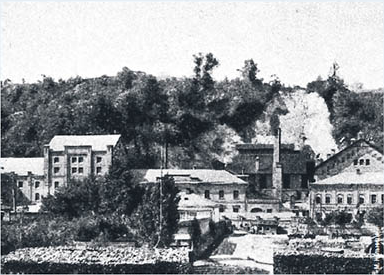
\includegraphics[width=\linewidth]{chast-kirvys/lys02/pivzavod-tov-02.png}

\textit{Конец 19 века, пивзавод Общества – справа, пивзавод Рихерта – слева, склон Лысой горы – позади во всей красе.}
\end{center}


\begin{center}
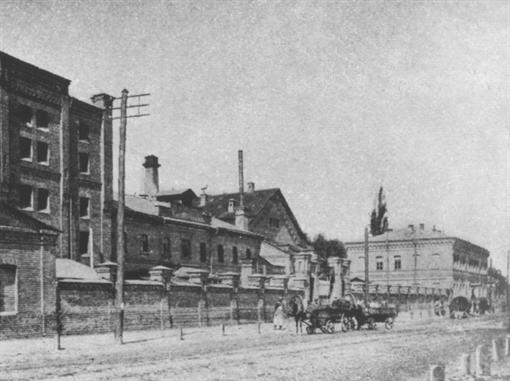
\includegraphics[width=0.95\linewidth]{chast-kirvys/lys02/1897-pivzavod-tov.jpg}

\textit{1897. Завод «Общества Киевского пивоваренного завода»}
\end{center}


Но вернемся к созданию пивзавода. В дело пошла часть корпусов прежнего, металлургического предприятия. Например, двухэтажная литейная стала варочным цехом. Новые же здания построили под машинное отделение, разливочную, солодовню. Николаев писал:

\begin{quotation}
В первый год моего пребывания в Киеве в 1872 году мною были построены здания наибольшего до сих пор в Киеве пивоваренного завода акционерного товарищества, причем в одно лето уложено было до четырех с половиною миллионов кирпича, и если в этой работе и мало можно найти художественных сторон, то в техническом отношении это была хорошая школа, как по громадности сооружений каменных, так еще главнее по грандиозности земляных работ, где приходилось для устройства ледников врываться в гору и вести нелегкую борьбу с массой стремившихся подземных ключей, причем вся распорядительная техническая сторона дела всецело лежала на мне. 
\end{quotation}

Воду сначала брали из городского водопровода, но затем выкопали колодец и варили пиво уже на основе колодезной. Оборудование заказали чешское, у «Шкоды», сырье – ячмень, хмель – поначалу завозили из Богемии и Баварии, затем перешли на отечественное, производство которого стало развиваться во многом для удовлетворения нужд отечественных пивоварен.

В советское время предприятие стало «Киевским пивзаводом №2» и продолжало работать. Великая Отечественная, немецкая оккупация. После восстановления в 1943-м, существовало по назначению до 2014 года, в последнее время как «ЗАО Пивзавод на Подоле». Летом 2014-го здания выставлены на продажу.

Позади завода Солодовых экстрактов и Пивзавода на Подоле, сбоку поля, под горой, в замусоренном котловане приютилось озеро, возникшее от заполнения очередного заводского глинища водой. Другие карьеры к нашему времени засыпаны. Я не спускался к воде, потому что когда мы снимали в том краю серию «Киевской амплитуды», шел проливной дождь, мы давно вымокли, да и крутой берег, превращенный в свалку, порядочно размок и лезть вниз не хотелось.

Между Пивзаводом на Подоле и Мыльным переулком, по адресу Кирилловская 49, в конце 19 века существовал еще один завод, Гриневича, выпускавший железные шкафы, медные трубы и паровые машины.

Итак, перед Лысой горой, между нею и улицами Нижнеюрковской да Кирилловской, уже много веков подряд действовали различные заводы, пожирая склон в ходе деятельности своей да в целях строительства. А ведь именно здесь, на месте срытого склона и его остатков, должен был стоять сотворенный летописными братьями град Киев – крепость, именованная в честь старшего брата, вероятно он ею и владел, ведь название указывает – чей град? Кия, Киев град. 

В сборнике «Чтения в историческом обществе Нестора летописца» (книга 1, 1873-1877, стр. 250) Антонович в примечании к статье «Археологические находки и раскопки в Киевской губернии 1876 г.» как бы между прочим рассуждает об этой местности:

\begin{quotation}
Окрестности Иорданской церкви в древности (в XI-XI столетии) составляли вероятно центр, в котором сосредоточивалась торговая деятельность города; в этой же местности найдены были все крупные клады Саманидских монет; там же, в соседней усадьбе (Товарищества пивоваренного завода) в 1870 году, оказалось огромное костилище, вмещавшее в себе около 4000 скелетов.
\end{quotation}

Иорданская церковь – на Мыльном переулке, под Лысой горой, прежде была чуть севернее, в 19 веке имела адрес Кирилловская, 51. Ну а про усадьбу Товарищества, или общества, пивоваренного завода – Пивзавод №2 – мы уже всё знаем.

Казалось бы, удивительная, важнейшая археологическая находка – 4000 скелетов! А сведений о ней – никаких, кроме еще двух заметок того же Антоновича. Первая из них содержится в тексте доклада 1877 года «О древнем кладбище у Иорданской церкви в Киеве»:

\begin{quotation}
Кроме того, несколько лет назад, разрывая один склон горы, нашли большую полость, наполненную огромным количеством костей – мужских, женских и детских, с небольшим количеством при них вещей, сваленных в большую яму; всего до 4000 черепов, – вероятно это были жертвы насильственно истребленные при разрушении этой части города.
\end{quotation}

И в «Археологической карте Киевской губернии»\cite{antonovich01} 1895 года Антонович сообщает:

\begin{quotation}
в усадьбе товарищества пивоваренного завода, на склоне горы, найдено множество человеческих костей (более 2000 черепов), сваленных в кучу; среди них найдены: железные: 2 длинные, обо\-юдоострые прямые меча, кинжал, удила, нож с костяной зеленою рукояткою; бронзовые: перстень, серьга и 2 браслета, обломки стеклянных браслетов, стеклянныя и глинистыя бусы, крестики: мраморные и янтарный. Музей Киевского университета. Указатель выставки 20-21; заметки и коллекция Антоновича.
\end{quotation}

Здесь уже уточнения. Место – «на склоне горы». Количество тел уменьшено в два раза – какому же числу верить? В любом случае, даже 2000 скелетов, найденные вместе, заслуживают внимания со стороны ученых. А тут лишь три кратких сообщения об этом. Всё. Каргер в «Древнем Киеве»\cite{karger01} вспомнил про меч и предположил, что он 8-10 века.

\begin{center}
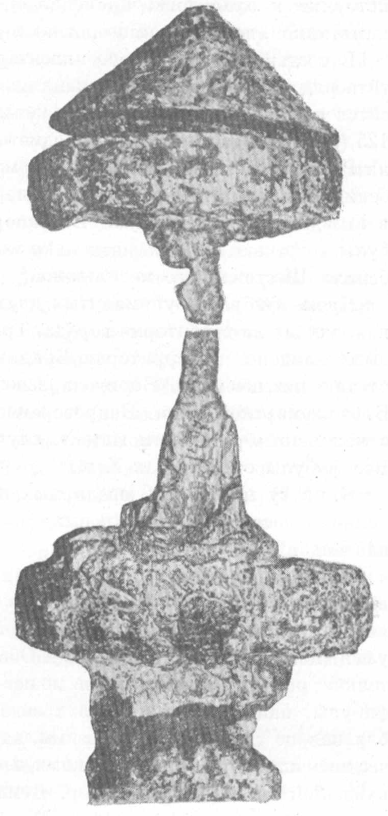
\includegraphics[width=0.45\linewidth]{chast-kirvys/lys02/4000-mech.png}

\textit{Рукоять меча, найденного вместе с останками. Инвентарный номер в Киевском историческом музее: 67192-1497.}
\end{center}

Причина смерти – убиты или умерли? В разное ли время? Ведь это может быть и кладбище, и могильник жертв побоища. В старину были еще скудельницы, божедомки – ямы, куда скидывали упокоившихся без причастия, самоубийц, бродяг и так далее. Наполнится яма – засыплют, потом роют рядом другую. 

Что значит «большая полость» – пещера? Найдена ли на скелетах одежда? А остатки гробов? Ничего неизвестно. К какому времени относятся упомянутые предметы, найденные среди скелетов? Помимо предположения Каргера о возрасте меча.

В любом случае, пусть 2000, не 4000 черепов, свидетельствуют о существовании крупного по давним временам поселения, причем именно там, где, по миниатюре Радзивилловской летописи, находится град Киев!

Мы уже знаем, что здесь были городища, курганы, а теперь еще и массовое захоронение возможно более близкого к нам времени, если меч – 8-10 века. Конечно, это давно обжитое место братья Кий, Хорив и Щек решили усилить и сотворить таким образом укрепленное поселение – град Киев, в честь старшего из братьев.

К сожалению, я пока не исследовал должным образом склон над «плато» и озером. Как понимаю, Антонович нашел кости, если определять место по современным ориентирам, на отрезке склона, где теперь пустырь у карьерного озера и до тупика Мыльного переулка. Туда можно добраться двумя способами – сверху от улицы Отто Шмидта, преодолевая все террасы, либо низом, вдоль склона, от современной Иорданской церкви-новодела в конце Мыльного переулка. Последнее мы показали в фильме «Логово Змиево», а местность сверху – в «Возвращение в Логово Змиево».

Уцелевшая часть восточной стороны Лысой горы, у подножия которой по горбам идет замусоренная тропка, переходит в поросшее травой плато, огромный пустырь, граничащий с упомянутыми тремя заводами да озером. Склон спускается к полю не постепенно, а небольшими глинистыми обрывами, из которых сочится влага, превращая всё под обрывом в вязкое месиво (мне кажется, я увидал там кости мамонта, однако не смог подобраться ближе). Раньше этот склон был выдвинут в сторону улицы Кирилловской почти на один уровень с соседней Щекавицей.

Что же исследователи – археологи, историки? Придают ли они значение огромному количеству человеческих останков? Как освещен этот вопрос в литературе? Редко упоминают об этих костях, не более, чем сам Антонович. Еще и пивзаводы путают. 

Считаю страшную находку Антоновича одним из главных доказательств существования «сотворенного братьями» града Киева именно на Лысой горе.

Есть ли еще тому подтверждения? Курганы, городища, огромное захоронение – чего же боле? Но есть и боле. Пойдем дальше по улице Кирилловской.

Вот мы добрались до Мыльного переулка. Сначала кратко, что и как здесь было.

Ныне переулок уходит по бывшему глинищу вглубь вдоль уцелевшего северного отрога Лысой горы, между ним и южным. Кирпичный завод съел южный отрог, на его месте – плато. Между обоими отрогами добычей глины прожран громадный овраг. От Мыльного дальше по Кирилловской стояла Иорданская церковь, сейчас тут нотная фабрика (новая Иорданская церковь смещена внутрь переулка). Затем, однако до перекрестка с улицей Заводской – переулок Иорданский, на картах его нет, а на деле есть. Сразу за ним был «Винокуренный и дрожжевой завод Марр».

Мыльным переулком иногда считали и Иорданский, то есть оба, соединенные, носили общее имя. Для удобства повествования я разделяю эти переулки. Мнение, что Иорданский переулок – другое название Мыльного – ошибочно. Изначально, как видно по старым картам, в этой области улица Кирилловская пересекается тремя переулками – Мыльным, Иорданским и Богословским. Мыльный остался и сохранил имя, Иорданский сохранился, но потерял имя, а Богословский продлился и стал Богуславским спуском.

Мыльный переулок назвался от татарской мыловарни, обеспечивающей татар работой. Ведь к востоку по прямой от пересекающего Кирилловскую переулка была скотобойня, а где скотобойни, там и мыловарни, ибо сырьё. Смрадную бойню же сюда, на Плоскую окраину, перенесли с самого Подола, из окрестностей Борисоглебской церкви. Что до кожевников, или «кушнеров», то они жили в Плоской части издавна, по крайней мере с 18 века.

\begin{center}
\includegraphics[width=\linewidth]{chast-kirvys/lys02/\myimgprefix IMG_20130728_154324.jpg}

\textit{Иорданский переулок не обозначен на картах.}
\end{center}

Существует важный с точки зрения краеведения вопрос об Иорданском ручье, который то ли протекал вдоль Мыльного переулка, беря начало у оврага к западу, то ли Иорданским слыл другой ручей, поныне журчащий на северу от сего места, за автобазой у Богуславского спуска. Дело запутанное, поэтому вынесено мною в отдельную главу «Иорданский ручей».

Покамест примем за истину, что в этой местности протекал один или несколько ручьев и сочился некий источник на горе – неясно, связанный ли с этими ручьями, однако вода из него была по трубам проведена в колодец подле Иорданской церкви.

Кстати, на плане Ушакова 1695 года, перед Иорданским монастырем, с юго-восточной его стороны, нарисованы «Мостки на грязи». Наверняка эта грязь относится к ручьям около монастыря.

Мыльный переулок въедается в Кирилловские высоты, а позади нотной фабрики (здания 51/1, 51-А) громоздится вверх заросший кустами и цепляющимися за кручу деревьями склон отрога Лысой горы, приблизившейся тут к улице Кирилловской на расстояние двора этой фабрики. Мыльный как бы отклоняет гору прочь от улицы. 

Я пробовал залезть наверх возле фабрики, но потерпел неудачу, натолкнувшись в конце концов на совершенно непроходимый бурелом. Не советую повторять мой опыт – во-первых, проще обойти, во-вторых, есть риск основательно загреметь вниз, если под ногами посыпется суглинок или обломится ветка, за которую держитесь. А если не держаться, обязательно свалитесь.

Прежде, Мыльный переулок, перпенди\-кулярный Ки\-рилловской, продолжался и на четной ее стороне, вглубь нынешней глухой промзоны. Еще раньше этот отрезок Мыльного был отдельной, Иорданской (Мыльной) улицей. Она шла параллельно Чернечьей улице в направлении к скотобойне на берегу Чернечьего (Иорданского) озера.

Мыльный переулок огибал усадьбу церкви и  соединялся за нею с Иорданским переулком. Если встать лицом к нотной фабрике, прежнему месту церкви, слева от нас будет современный Мыльный. Он просто уходит вглубь, вдоль горы, что пыжится вверх сразу за нотной фабрикой. Поскольку тут гора неприступна, надо лезть сбоку, от современной Иорданской обители, либо по неприметной лестничке в Иорданском переулке.

Справа от нотной фабрики, между нею и соседней к северу фабрикой молочной кислоты\footnote{Кирилловская, 53. Фабрика выросла из пивзавода Марр.}, чуть вверх поднимается и загибается к юго-востоку Иорданский переулок. В точке его изгиба – лестничка\footnote{Около нее в 2015-16 годах велось строительство, рядом с развалюхой старенького одноэтажного домика. Таких домиков, вероятно, раньше здесь было больше.} к земляной дорожке, по которой можно выбраться в глубокий овраг между мысом Лысой горы и отрогом с дачами садового товарищества «Кожевник». 

По этому оврагу в старину проходила дорога на Лукьяновку (в тогдашнем понимании этого слова) - по словам Похилевича – Старый Никольский ввоз, а его низовье над нотной фабрикой лежит по уступам Иорданского кладбища, на склоне Лысой горы и лощине между нею и соседней горой «Кожевника».

Посмотрим на часть карты Меленского за 1833 год, где выше Рогаток подписана Юрковица, а правее, у необозначенной Лысой горы – Иорданская церковь и горное, разделенное надвое кладбище над нею:

\begin{center}
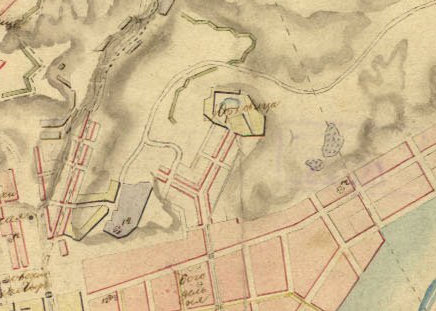
\includegraphics[width=\linewidth]{chast-kirvys/lys02/1833-melenskiy.jpg}
\end{center}

Это разделение кладбища послужило причиной моего предположения, что на отроге Лысой горы за Иорданской церковью была меньшая часть кладбища, а на отроге «Кожевника» – б\'ольшая, но сопоставление по положению церкви заставило меня пересмотреть взгляды и счесть всё изображенное на этой карте кладбище как относящееся только к отрогу Лысой. 

На других дореволюционных картах я видел кладбище только, кажется, на южном отроге. Однако на точнейшем плане РККА 1937 года кладбище явно занимает оба отрога.

Кусочек плана 1864 года, ориентированный как если смотреть на Высоты с улицы Кирилловской, хорошо показаны все отроги:

\begin{center}
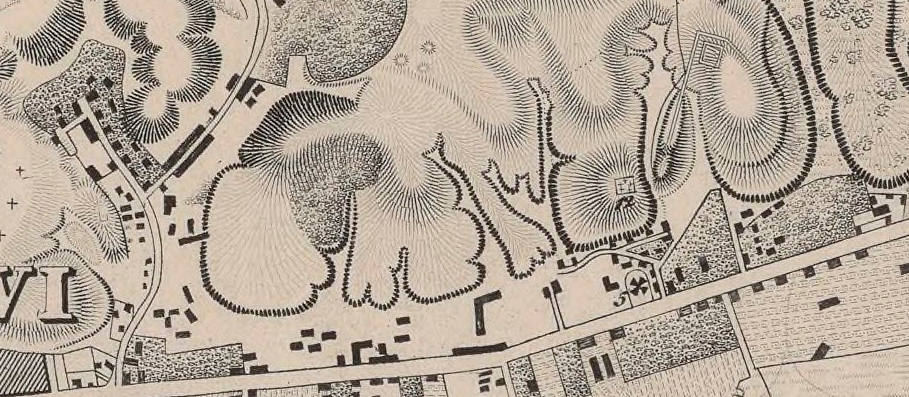
\includegraphics[width=\linewidth]{chast-kirvys/lys02/1846-y.jpg}
\end{center}

Узнаваемая Рогатка слева, затем еще полноценная, не срытая южная часть Лысой горы. Числом 5 обозначена Иорданская церковь, 12 – кладбище над нею. Видите, какие ровные очертания этого отрога? На нем и сохранились древние валы. Правее на отрожке, взбирающемся на мыс «Кожевника», нарисована странная прямая дорожка к прямоугольнику наверху. Что это? 

Местность сию нам надлежит изучить внимательно, постепенно погружаясь в прошлое. Рассмотрим, один за другим, источники.

Впервые Иорданская церковь возникает в документах 17 века, как церковь «святого Миколы Иорданского», окруженная урочищами, чьи названия давно исчезли и уже трудно определить, что им соответствует ныне.

Жалованная грамота Киевского воеводы, князя Константина Острожского, предоставляющая во владение земянину Войтеху Соколовскому в предместье Киева «пляц с огородами на месте пустом» и сеножать, называемую Пунища, 1602, апреля 12:
\begin{otherlanguage}{polish}
\begin{quotation}
dalismu iemu placz z ogrodami na mieyscu pustem, gruncziku w Kyiowie, na przedmiesciu, a ku themu sianozenczi, nazwane Puniscza z niwami, z dabrowami, przy nim naliezaczemi, przy tym ze Borki y ze wszystkimi przynalieznoscami do nich; do tego przydalismu iezioro y za piassoczmi przy nim naliezaczemi nazwane Kossor, nad rzeka Dnieprzem, do laski iego krolewskiej mosci, ktory to pliacz i z ogrodami grunciku poczyna sie od walku, konczy sie \textbf{u potoka cerkwie s. Mikoly Jerdan\-skiego}, a z drugiey strony od drogi, ktora ydzie z miasta od nowey bassty ku Demidowu, (do) drogi gostincza Bialogrodzkiego, na kturom to gostinczu wolno iemu wszelakie pozytki
\end{quotation}
\end{otherlanguage}
«У потока церкви святого Миколы Ерданскего». Речь идет о неуловимом Иорданском ручье или потоке, что ныне шумит в коллекторе вдоль северо-западной стороны отрога, где теперь дачи садового товарищества «Кожевник». Последний ручей использовался Иорданским монастырем для всяческих нужд и устройства пруда.

Вариант документа о владении Войтеха Соколовского находится в «Выписи с книг кгродских воеводства Киевского», от 14 июня (Акты Южной и Юго-западной Руси, том 2, стр 15):

\begin{quotation}
пляцу з огородами у Киеве на передмесстю и сеножать, названую Пунища, з нивами, з дубровами, при них лежачими, также в Борки и во все приналежности и в езеро за песочьем названое Косор (Косур в списках) над рекою Днепром.
\end{quotation}

Третий вариант:

\begin{quotation}
на данье пляцу в пусте лежачого на предместю Киевском, недалеко от церкви светого Николы Ерданского, и к нему сеножати названое Пунисчь и з нивами к ней належачими, кгрунту теж у пусте лежачого названого Борки и озеро Косор.
\end{quotation}

Четвертый:

\begin{quotation}
пусто и без всякого пожитку лежачий пляц з огородами у Киеве на передместю, а ку тому пляцови пустому сеножать, названую Пунисча з нивами при ней лежачими, который то пляц кгрунтику с тыми огородами починается от валку а кончитьсе у потока при церкве светого Николы Ерданского, з другое стороны от дороги, которая идет з места ку Демидову до дороги гостинца Белогородского [...]

к тому ж вышей помененому кгрунтикови также пусто лежачий кгрунтик и озерцо речоные Борки, Косор за песочем над рекой Днепром лежачее
\end{quotation}

Урочище Пунище я показывал на карте 1752 года, в главе про Почайну. Сохранились документы со сведениями, что Пунища и «грунт» Соколовского подвергались нападениям монахов Кирилловского монастыря, а на грунте шляхтича стоял кирпичный завод. 

%Надо полагать, завод сей не в чистом поле Оболони, а именно возле горы, близ Иорданской церкви. Стало быть и Пунища рядом. Борки и Косор требуют тщательного изучения. Но озеро Косор (Косар), кажется, лежало несколько севернее, ближе к Вышгороду. Для меня важно, что основной «грунтик» Соколовского был возле Иорданской церкви.

Получив землю, Войтех Соколовский приобрел и забот полон рот. Уже летом 1608 года Соколовский жалуется властям на игумена Кирилловского монастыря, Василия Красовского, по прозвищу Чернобровка.

Монастырская братия напала на работников Соколовского, которые на волах пахали ниву Пунищу. Побили работников – Самоила и Яцка – а волов купно с сохами и ярмами угнали и присвоили в пользу монастыря, не забыв похитить также топор и две сермяги. 

Пока около года шли жалобы, монахи успели спалить на Пунищах два стога сена (по 15 возов каждый), и разрушить кирпичный завод Соколовского, состоящий из сарая с печью – в нем же хранились готовые кирпичи. Бесчинствующая братия уничтожила и оные кирпичи, числом примерно 10 тысяч штук. Особенно усердствовали слуги игумена, Андрейко да Богдан.

С лета 1609 начались судебные разбирательства.

Вдруг оказалось, что «грунты», полученные Соколовским, были вовсе не пустыми и ничейными, а принадлежали Кирилловскому монастырю, и что Соколовский прогнал оттуда некоего «оселого на имя Онтона» и захватил земли Кирилловские и Ерданские со строениями, включая церковные, кои принялся разбирать и употреблять на строительство своего дома. Проломив дыру в церковной стене, Войтех Соколовский «власными руками» вытащил замурованный там сундук с пожертвованиями на 50 тысяч золотых червонцев. Что против этого битые работники да кирпичи?

Тяжба длилась годами. В 1612 году Соколовский умер и его земли под Киевом (те ли, спорные?) достались по наследству родственникам, и далее судьба части владений (Пунище, Косар) иногда всплывает в земельных документах.

Иорданская Николаевская церковь того времени, судя по всему, была каменной, то бишь кирпичной, ибо Соколовский учинил «ломанье муров, выбинье цеглы, плиты, каменя церковного». Когда её построили, мне неведомо. Соколовский превратил храм в строительные материалы. Возможно, он стоял в запустении и никто им не пользовался по назначению.

Возрождение наступило несколько позже. По Максиму Берлинскому, девичий монастырь при храме завели в 1616, а по сведениям поручика Новгородцева – в 1650 году. Новгородцев однако ошибается, поскольку в Львовской летописи мы находим, за 1630 год, следующее:

\begin{quotation}
На третий день тыиж Немцы Иорданскии под Киевом монастырь пошарпали и до Межигорского монастыря хтели штурмовати.
\end{quotation}

Значит, в 1630 году монастырь уже существовал. Далее он упомянут в «Росписи Киеву» за 1682 год:

\begin{quotation}
в том нижнем городе Кожемяцкие ворота в Шкавицкой горе; Ерданские ворота, ездят к Ерданскому и к Кирилловскому монастырем.
\end{quotation}

На плане 1752 года, вдоль горы на северо-запад рядом с Иорданским монастырем показан Богословский. 

В «Географическом описании града Киева» за 1784 год, поручика Новгородцева, Богословский тоже стоит по соседству с Иорданским: 

\begin{quotation}
А при Киево-Подоле ведомства Кириловского монастыря смежна слобода, называемая плоская в которой есть два девичих Богословский и Иорданский монастыри. Далее за оной слободой в разстоянии от Подола 2-х верст: Кириловский мужеский монастырь. [...]

10. Киево-Иорданский девичий монастырь. В нем церковь святителя Христова Николая с одним престолом. Оный монастырь построен с 1650 года [...] 

В оном монастыре монахинь, келейниц, послушниц и служителей 217. В том же монастыре трапеза 1. Келии игуменския, и, для монашествующих, деревянных 108. Вокруг сего монастыря ограда с колокольнею, деревянные.

11. Киево-богословский девичей монастырь. В нем соборная церковь, во имя святаго Иоанна Богослова об одном престоле. Сей монастырь, называемый Свято-Софиевским девичьим монастырем, построен был благоверною царевною Софиею Александровною; имел свое положение в старом верхнем городе Киеве, через одну токмо стену с мужеским киево-золото\-верхо-михайловским монастырем, в котором девичьем монастыре храм устроен был в честь оной царевны, то есть св. великомуч. Софии и трех ея дочерей: Веры, Надежды, Любви. 

В котором же году был оной монастырь там построен, за сгорением по случаю пожара письменных документов, справиться не по чему. 

А в 1711-м году, по повелению блаженной и достойной памяти Государя Императора Петра Первого, переведен на настоящее место, и устроена при оном казенным коштом церков деревянная во имя святаго Иоанна Богослова. В оном монастыре монахинь, келейниц, послушниц и служителей 126. В том же монастыре теплая трапезная церковь во имя святых праведных Захарии и Елисаветы, об одном престоле деревянная. Келии, игуменския, и для монашествующих деревянные 55. Вокруг монастыря, ограда с колокольнею деревянные.
\end{quotation}

Точное местоположение Богословского монастыря мне неведомо. На плане 1752 года он нарисован на северо-запад от Иорданского монастыря, чуть дальше по склону.

Антонович под конец 19 века в неких руинах в окрестностях Богословского переулка (где именно – неясно) предполагал остатки сего монастыря. Их же, вероятно, видел первый киевский археолог Кондрат Лохвицкий, ибо привязывал к оным обнаруженные им другие развалины. На этом же участке – назовем его условно «усадьбой Марр» – в 1947 году археологи обнаружили фундамент «древнерусского храма», но подробности мне неизвестны. Древнерусское к Богословскому монастырю не относится.

Петр Первый переместил на окраины два монастыря. Первый это Флоровский, связанный с именем матери Мазепы, столь нелюбимого Петром. Царевна Софья также была в опале. С другой стороны, причиной переноса монастырей могла быть не личная неприязнь Петра Первого, а желание отдалить женские обители от мужских.

Богословский монастырь возникает на Кирилловских высотах как явление временное. В 1789 году его монахинь перевели, как и жительниц Золотоношского Благовещенского монастыря, на  Красную горку, и там образовался, на месте бывшего мужского Преображенского монастыря, Покровский Золотоношский Красногорский женский монастырь, закрытый в 1923 году и возрожденный в ноябре 1941 года во время немецкой оккупации. 

Закревский в своей книге ошибочно указывает, что Иорданский и Богословский монастыри соединились в один Иорданский. Ошибается и Берлинский, говоря про объединение монастырей в 1712 году. Этому противоречит карта 1752 года, и сведения 1786 года, согласно коим каждый монастырь отдельно предоставлял в консисторию (совет при архиерее по управлению епархией) донесения. «Настоятелькой» Иорданского была мать Александра, а Богословского – Ксанфия.

Деревянные кельи, о коих Новгородцев сообщает при описании монастыря, обозначают не комнатки в каком-то монашеской общежитии, а небольшие домики. Они соседствовали с селом Плоским, славящимся своими винокурнями да шинками.

Иорданский и Богословский монастыри, в отличие от, как бы сейчас сказали, престижного Флоровского, являлись общинами более хозяйственными, чем духовными. Работали во всех трех, но во Флоровском жило много монахинь знатного происхождения, освобожденных от труда. 

Женские монастыри, по сути, были фабриками. Чем же занимались их обитательницы? Кроме ведения внутреннего хозяйства, это, в первую очередь, рукоделие. Если монастырь владел доходными промыслами, то зачастую сам же ими торговал, например столько-то монахинь выделялось на продажу мёда, свечей. 

На 1777 год в Иорданском монастыре было 98 монахинь и 10 белиц (жительниц монастыря, не постриженных в монашество, название противоположное «черницами»), а в Богословском – 52 монахини и 5 белиц. Для сравнения – в том же году во Флоровском насчитывалось 123 монахини и 8 белиц. Процент грамотных монахинь в Иорданском был выше, чем в Богословском.

Неясно мне, почему в 1786 году крепкий хозяйственный монастырь Иорданский был упразднен, а Богословский переведен в другое место. Почему оставили именно и только Флоровский? Иорданский, пусть и несколько отдаленный от насыщенного жизнью Подола, всё же был известен дольше, славен больше, да имел особенность, привлекающую паломников – легендарный чудодейственный источник. И кому досталась земля и постройки на ней Богословского монастыря, что с ними случилось? Не знаю.

Максим Берлинский в «Кратком описании Киева» 1820 года сообщает:

\begin{quotation}
Самая отдаленнейшая к северо-западу от Подола, на так называемой Плоской слободе, у подошвы горы находится деревянная церковь святителя Николая, теперь приходская. С 1616 года заведен был при сей церкви девичий монастырь Иорданский, названный так по чудесному случаю найденного в тут находящемся колодце серебреннаго котла который потерян был в реке Иордане в Палестине. 

Как бы то ни было, но монастырь сей уничтожен в 1786  году, и оставался как заштатный, пока существовали монахини. В соседстве его до того же времени существовал с деревянною же церковию другий девичий монастырь Богословский, который, как вышеупомянуто, сюда в 1712 году переведен от соседства Золотоверхо-Михайловского мужеского монастыря.
\end{quotation}

«Заштатный монастырь» значит, что монастырь был предназначен для закрытия, оставшись вне штатов. В ходе церковной реформы 18 века, Екатериной II была проведена секуляризация – изъятие земель из монастырских владений в пользу государства. Купно с землями отобрали и крестьян, которые вместо барщины смогли теперь платить оброк. Ввели понятие монастырских штатов с разделением монастырей и епархий на классы в зависимости от величины. 

Грубо говоря, штат – положенные по закону сотрудники духовного звания. Чем ниже класс, тем меньше в монастыре могло быть лиц. Например, в мужском монастыре 1-го класса – 8 иеромонахов, а 2-го класса – только 6. Все числящиеся по штату люди получали от государства пособие. Размер его зависел от класса. В женском монастыре 2-го класса игуменья получала 60 рублей, а 3-го класса – только 40. После Екатерины II эти суммы пересматривались.

Во второй половине 19 века, Иорданской церковью привычно называли уже не сгоревшую церковь святого Николая, а другую – Дмитрия. Похилевич в книге 1865 года «Монастыри и церкви Киева» помещает о ней важнейший раздел:

\begin{quotation}
Иорданская Димитриевская, в той же Плоской части подола, под горою, на северной оконечности Киево-Подола. В давнее время в этом месте был съезд с горы от Лукьяновки, следы которого и теперь еще приметны. 

Из рассмотрения местности и по остаткам щебня видно, что первоначально, еще до разорения Киева, Николаевский женский монастырь, упоминаемый в летописях, существовал на уступе горы, или на самой горе, где ныне две могилы и небольшое замковище и где в 1863 году случайно отыскан, при копании могилы для покойника, клад с серебянными арабскими деньгами и несколькими вещами.

Известно из жизнеописания преподобного Феодосия Печерского, что мать его была пострижена в сем Николаевском монастыре\footnote{С таким же успехом в летописи речь могла идти о Никольском монастыре, возникшем вокруг церкви святого Николы на Аскольдовой могиле. Что и к Лавре, где обитал Феодосий, гораздо ближе.}.

В начале XVII столетия Николаевский женский монастырь, в зависимости от мужеского Кириловского, возобновлен с присвоением название иорданского, которое, по преданию, присвоено монастырю от того, что какой-то Русский поклонник святых мест, уронив в реке Иордан близ Иерусалима серебрянный ковш, нашел его, возвратившись в Киев, в монастырском колодце, существующем и ныне на уступе горы, выше нынешнего церковного погоста, из которого проведена трубами превосходная вода в нижний, близ нынешней церкви.

В Иорданском монастыре главная церковь была во имя святителя Николая, которая в 1808 году, во время упразднения монастыря, была деревянная, о трех куполах, однопрестольная, на каменном фундаменте, с весьма хорошим и богатым украшением. Иорданский монастырь, к коему в 1712 году переведен и женский Богословский от Киево Михайловского, предположен был к закрытию еще при введении штатов в 1768 году; но по многолюдству женской общины существовал до 1808 года. 

При нем состояло два священника, диакон и три штатные служителя; а в пособие на содержание его, по имянному Высочайшему повелению 17 октября 1788 года, отпускалось из казны до самого его закрытия:
а) жалованья на 15 монахинь по 10 р. – 150 р.
б) двум священникам, каждому по 20 р. – 40.
в) двух церковникам по 10 р. (за них 1 диакон 20 р.)  – 20.
г) на просфоры и на дрова – 30.
д) на ремонт монастыря и ризницы – 50.
е) трем штатным служителям по 8 р. да прибавочных на муку и соль по 6 р. 22 1/2 коп. всего  – 42 р. 67 1/2. Всего в год монастырю – 332 р. 67 1/2 к.

При закрытии монастыря Николаевского в нем находилось до 100 монахинь и послушниц в 80 деревянных домиках, по горе раскиданных, которые большею частию принадлежали им как собственность, переходившая от одной монахини к другой независимо от церковного начальства.

Николаевская монастырская церковь, обращенная в приходскую, сгорела во время пожара 1821 года от соседнего кирпичного завода, находившегося до 1826 года на юг от церкви. Нынешняя Димитриевская деревянная церковь, построенная в половине прошлого столетия, считалась при существовании монастыря, трапезною. Штат ея с 1843 года состоит из священника, дьячка и пономаря. 

Домы церковные для причта остались еще от монастыря; большая же часть проданы монахинями частным лицам. Прихожан обоего пола 1480; сверх того в приходе живут: 16 раскольников и 41 лютеран и Римских католиков. Доход свечной и венчиковый простирается в год до 60, кошельковый и кружечный до 800 рублей.
\end{quotation}

Похилевич говорит о церкви святого Николая, что она деревянная на каменном фундаменте. Ранее я предположил, что в 17 веке шляхтич Соколовский разбирал каменную церковь. Как бы ни было, но в 1821 году (дату эту я подвергну сомнению позже) сгорела уже деревянная церковь Николая и главной временно стала деревянная Димитриевская, или Дмитрия Солунского, ранее бывшая трапезной. Где именно находилась сгоревшая церковь Николая? И где деревянная Димитриевская?

В 1884 году по Мыльному переулку, там где сейчас нотная фабрика, возвели новую, уже каменную церковь Дмитрия Солунского – кажется, несколько юго-восточнее прежней деревянной.

\begin{center}
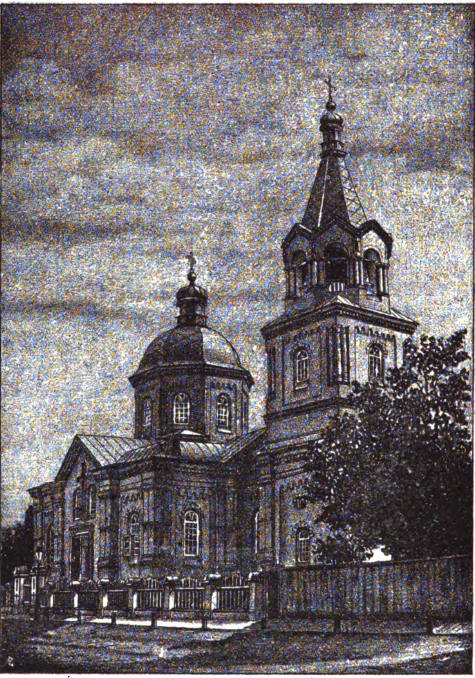
\includegraphics[width=0.70\linewidth]{chast-kirvys/lys02/1888-zaharchenko-iordan.jpg}

\textit{Иорданская Дмитриевская каменная церковь, иллюстрация из книги Захарченко, 1888 год.}
\end{center}

\newpage

\begin{center}
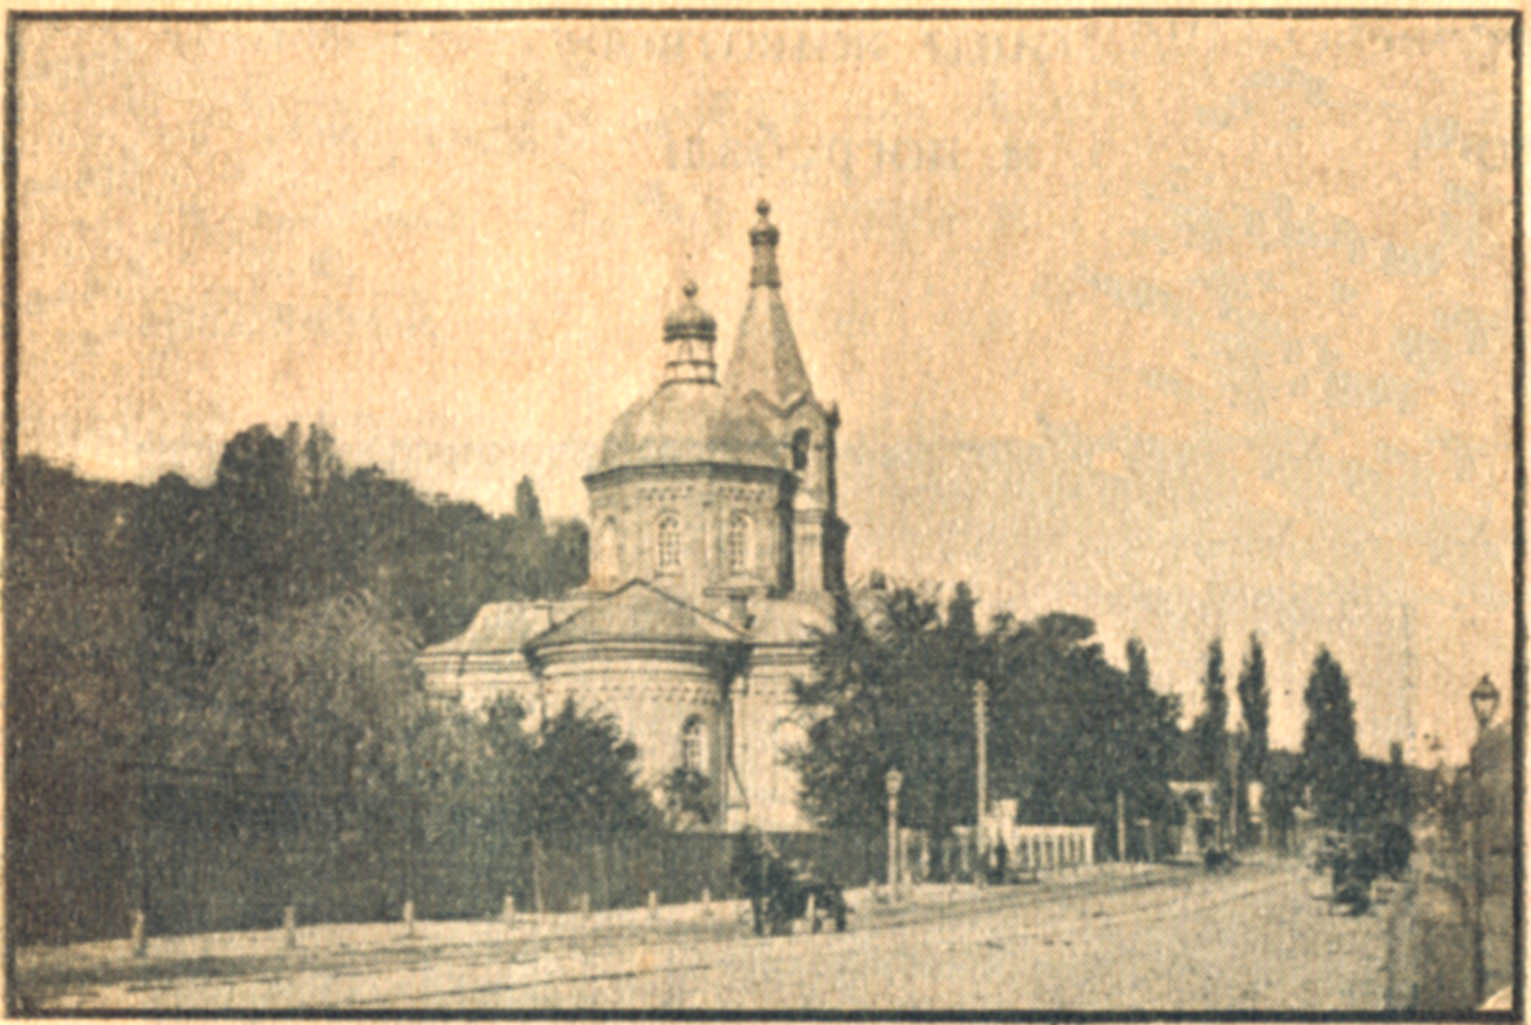
\includegraphics[width=\linewidth]{chast-kirvys/lys02/iordanskaja_cerkov.jpg}

\textit{Иорданская Дмитриевская каменная церковь, дореволюционный снимок.}
\end{center}

Эту каменную церковь, слывущую в народе просто Иорданской, разобрали в 1935-м и на её фундаменте построили школу. Во времена оккупации Киева фашистами она стала тюрьмой для советских военнопленных. Затем, в мирное время, в здании поместилась нотная фабрика.

Вернемся к Похилевичу и обсудим некоторые его важнейшие сообщения. Первое:

\begin{quotation}
В давнее время в этом месте был съезд с горы от Лукьяновки, следы которого и теперь еще приметны.
\end{quotation}

Следы были приметны при Похилевиче, приметны они и в 2020 году. «Съезд с горы» – тропа в овраге между двумя холмами: Лысой горой и дачами «Кожевника». Ширина оврага и плоское дно дает основания полагать, что тут раньше была хорошая дорога. Восходя ею, можно понять, каким был увоз Боричев – дорога не прётся в кручу, а плавно прорезается через нее, делая подъем пологим. Старинные кирпичи здесь не редкость, лежат грудами, как, впрочем, и множество иного, более современного мусора.

\begin{center}
\includegraphics[width=\linewidth]{chast-kirvys/lys02/\myimgprefix IMG_4375.JPG}

\textit{Остатки давней дороги в 2015 году.}
\end{center}

Похилевич пишет:

\begin{quotation}
Известно из жизнеописания преподобного Феодосия Печерского, что мать его была пострижена в сем Николаевском монастыре. 
\end{quotation}

В житии Феодосия Печерского сказано, что мать Феодосия отправилась в «монастырь женский, именуем святаго Николы» и была там пострижена. Однако никаких уточнений относительно местоположения его нет.

\begin{quotation}
Из рассмотрения местности и по остаткам щебня видно, что первоначально, еще до разорения Киева, Николаевский женский монастырь, упоминаемый в летописях, существовал на уступе горы, или на самой горе, где ныне две могилы и небольшое замковище и где в 1863 году случайно отыскан, при копании могилы для покойника, клад с серебянными арабскими деньгами и несколькими вещами.
\end{quotation}

«Уступ горы» – возможно, терраса между верхом Лысой горы и нотной фабрикой. Там сохранились остатки Иорданского кладбища. На самой же горе при Похилевиче было «замковище». «Ище» добавляется к слову, дабы обозначить нечто оставленное, заброшенное. Скажем, монастырище – оставленный монастырь, его развалины. Подразумевал ли Похилевич под «замковищем» остатки деревянной или каменной крепости? Известны древнейшие \textbf{городища}, обычно на вершинах холмов, как раз вроде отрогов Кирилловских высот. Такие городища имели рвы и валы в части, примыкавшей к «материку». И ныне наверху Лысой горы – странные древние рвы и валы, пересекающиеся под прямым углом. Однако рва или вала, защищающего мыс со стороны материка, я не видел. Это не означает, что его не было или нет. Просто холм там уже застроен.

Некие «перекопы и ровы» на Лысой горе упомянуты еще в «Решении о разграничении земель города Киева» 1701 года, где сказано, что перекопы и рвы устроены, дабы оградить проникновение городских стад на пастбище на горе. Но основной из древних рвов, о которых я говорю, никак не может быть к ним отнесен, поскольку примыкает к верху южного склона отрога.

\begin{center}
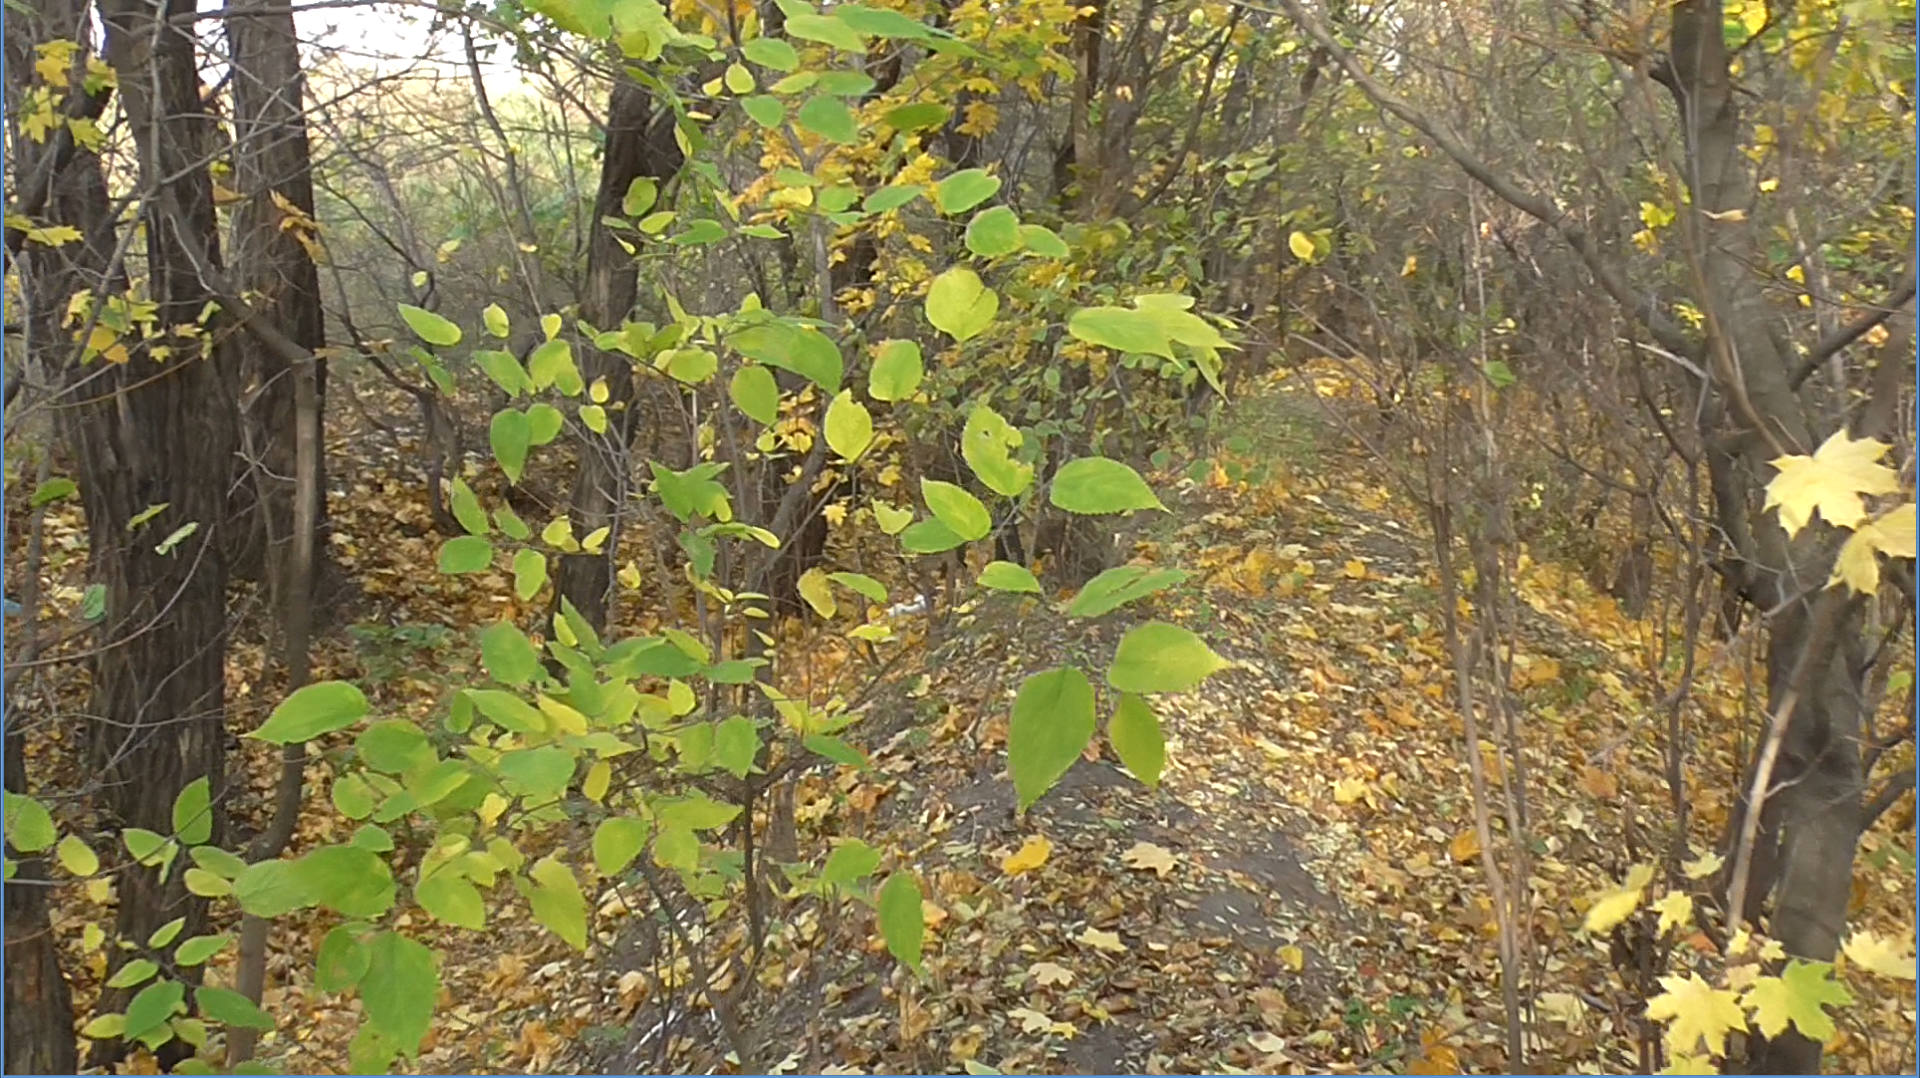
\includegraphics[width=0.95\linewidth]{chast-kirvys/lys02/lg03.jpg}

\textit{2013. Вал со рвом по юго-восточному склону отрога.}
\end{center}

\newpage
\vspace*{\fill}
\begin{center}
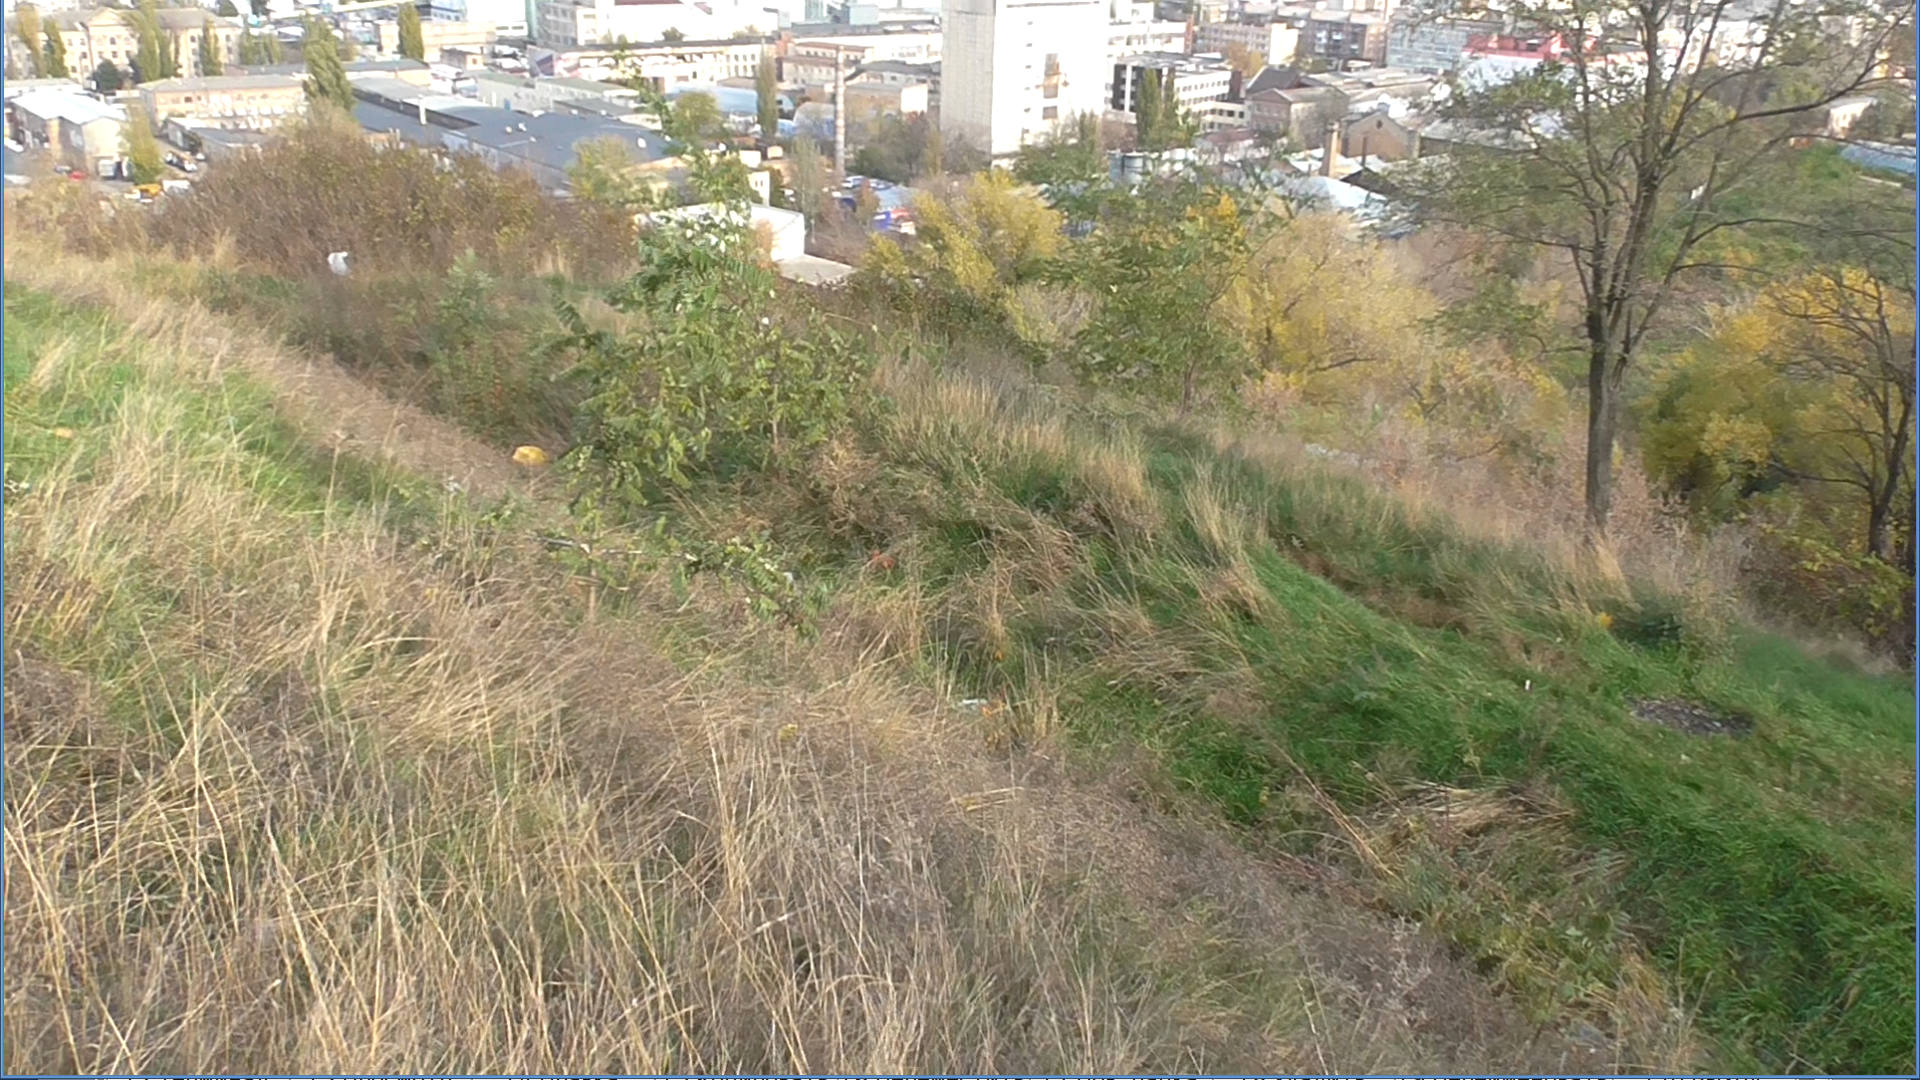
\includegraphics[width=\linewidth]{chast-kirvys/lys02/lg02.jpg}

\textit{2013. Юго-восточный склон, над Мыльным переулком (он справа).}
\end{center}

\begin{center}
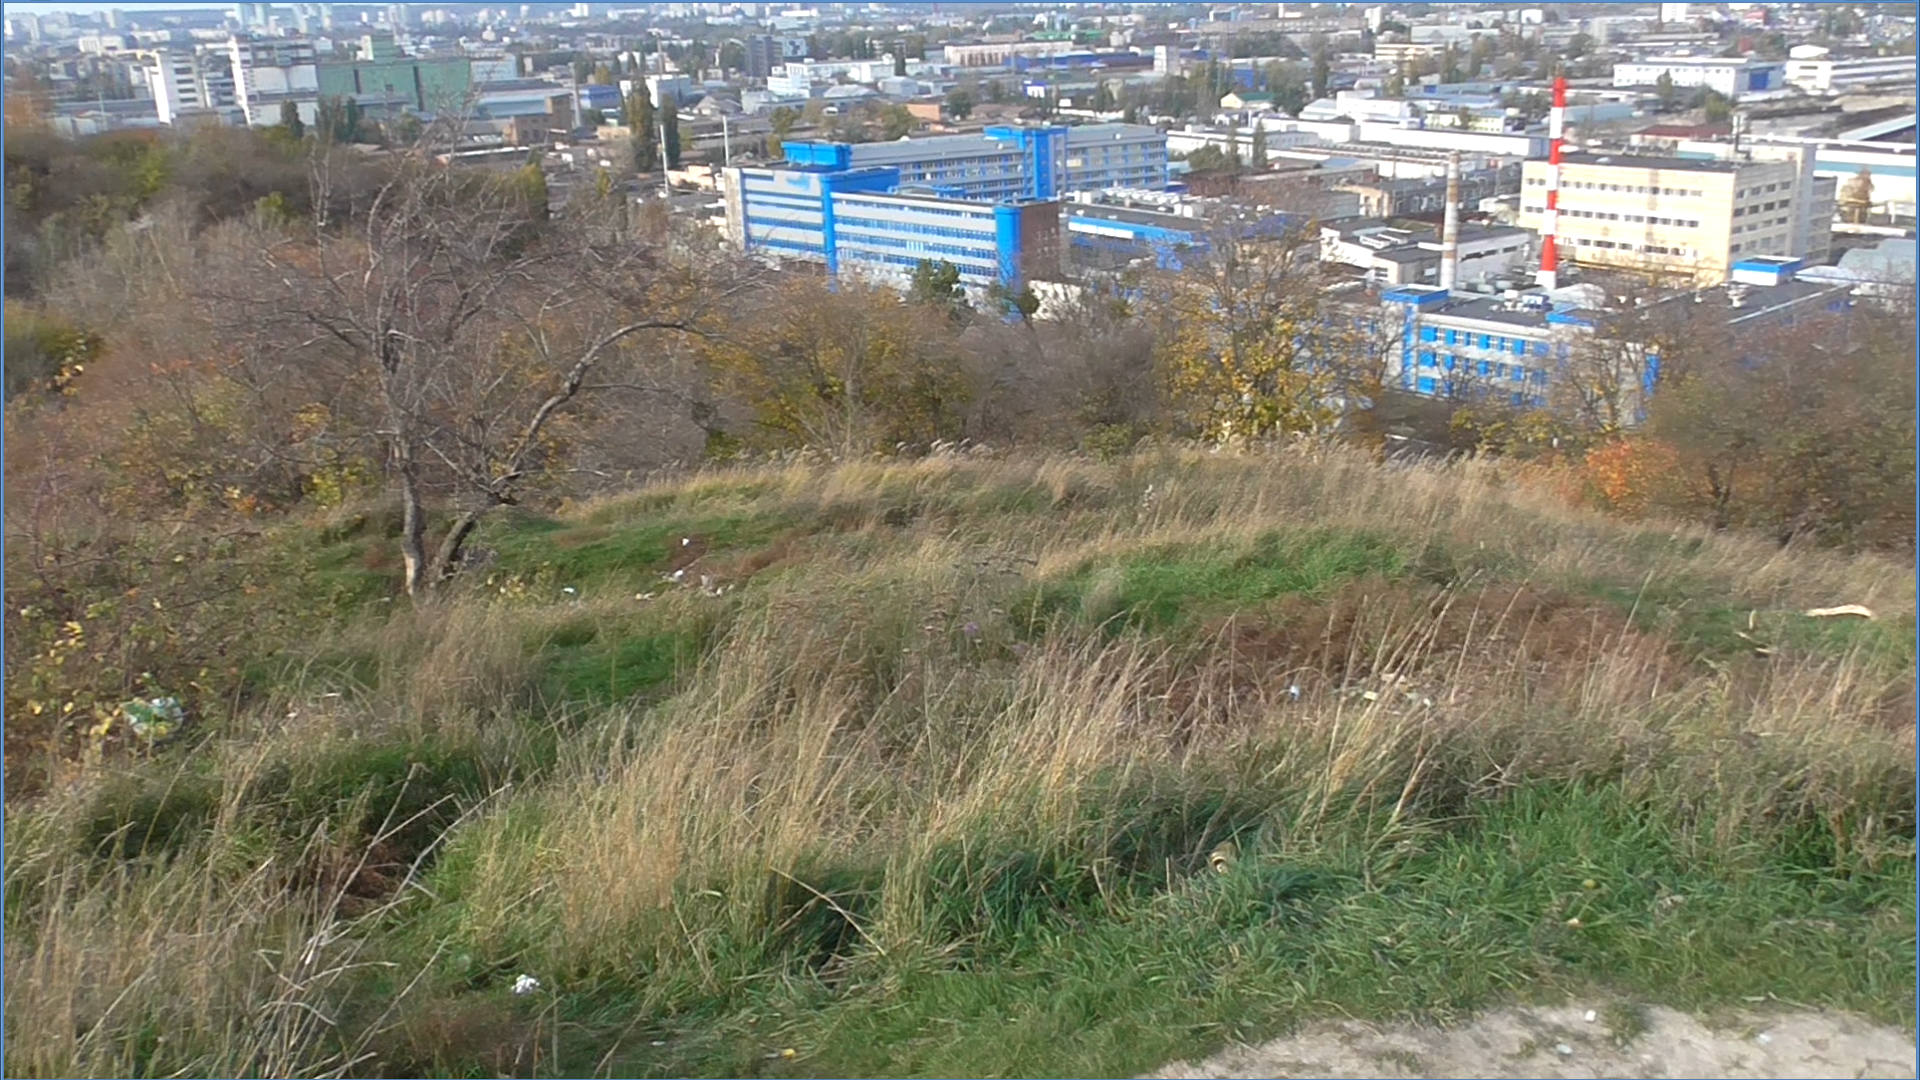
\includegraphics[width=\linewidth]{chast-kirvys/lys02/lg01.jpg}

\textit{2013. Край северо-восточного склона Лысой горы, к западу от Мыльного переулка.}
\end{center}
\vspace*{\fill}
\newpage

\newpage
\vspace*{\fill}
\begin{center}
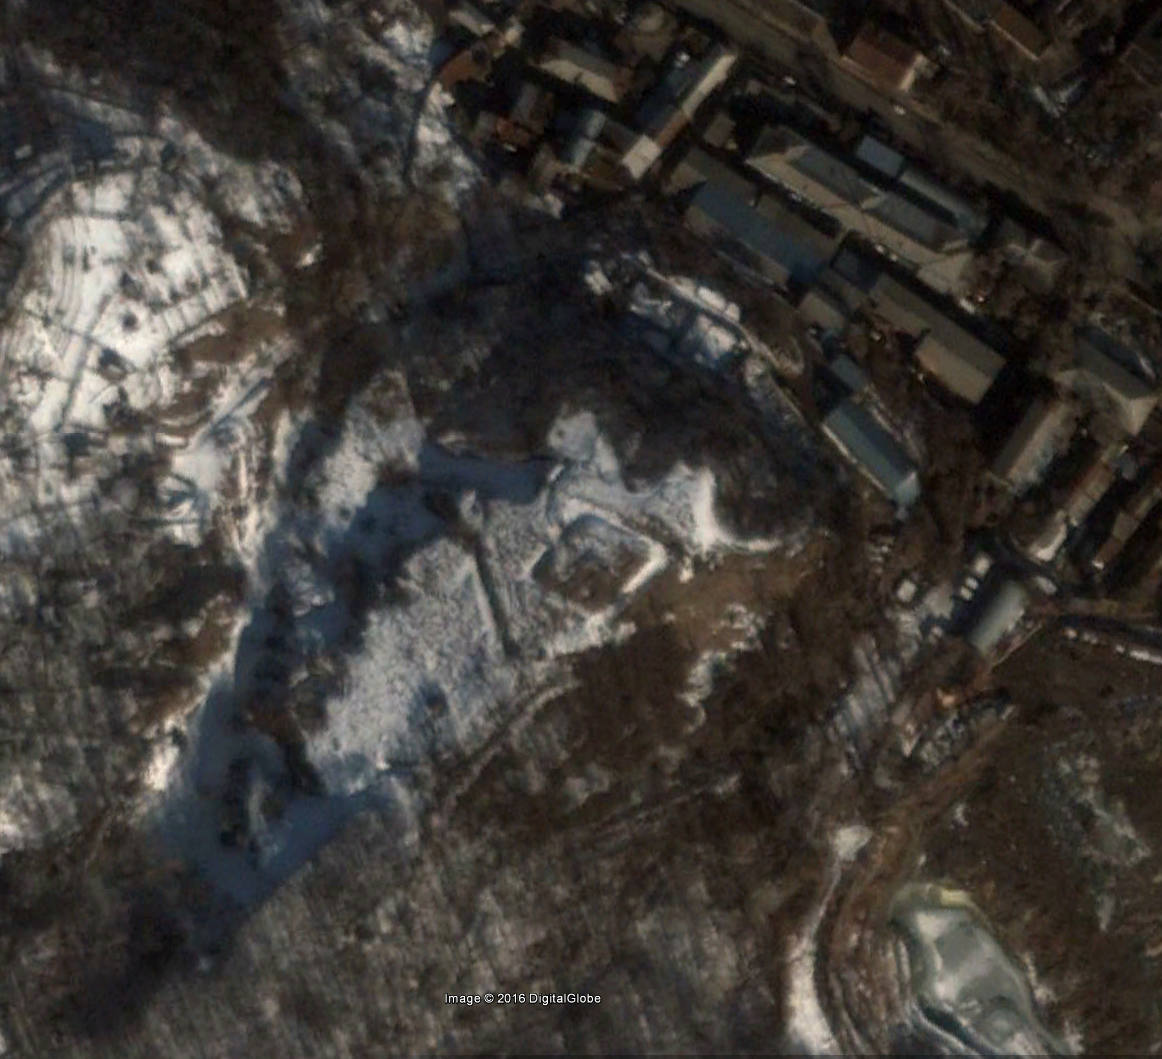
\includegraphics[width=\linewidth]{chast-kirvys/lys02/romb.jpg}

\textit{2001, спутниковый снимок. Городище – «ромб в треугольнике». Справа Мыльный переулок, слева терраса Иорданского кладбища и давняя дорога на Лукьяновку, в овраге. Однако на 1930-е кладбище занимало и верхнее плато с городищем.}
\end{center}
\vspace*{\fill}

\newpage

\newpage
\vspace*{\fill}
\begin{center}
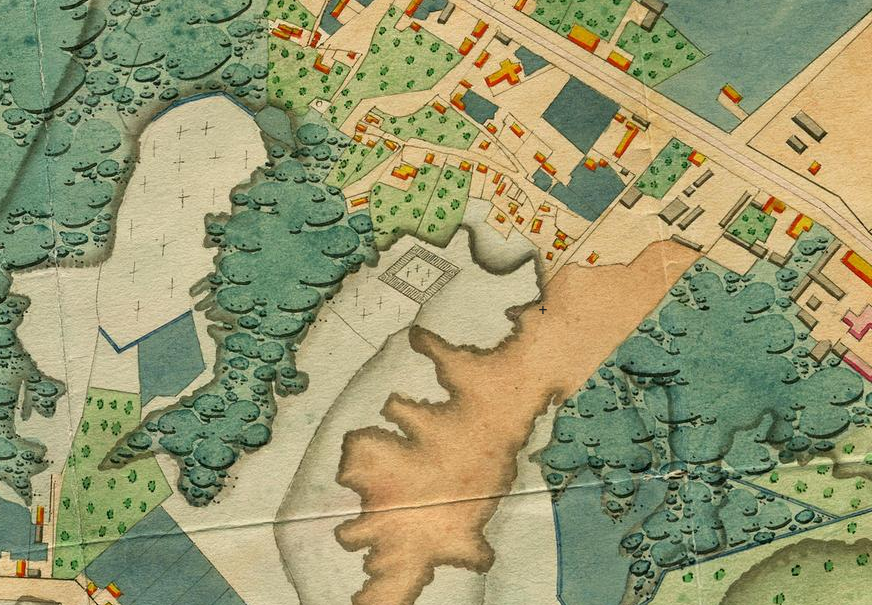
\includegraphics[width=\linewidth]{chast-kirvys/lys02/romb-1850.png}

\textit{1850-60, тот же странный ромб на кладбище.}
\end{center}
\vspace*{\fill}

\newpage


\begin{center}
\includegraphics[width=\linewidth]{chast-kirvys/lys02/\myimgprefix IMG_4345.JPG}
\end{center}

\begin{center}
\includegraphics[width=\linewidth]{chast-kirvys/lys02/\myimgprefix IMG_4354.JPG}

\textit{Вид на северо-западный склон Лысой горы с «замковищем» и Иорданским кладбищем.}
\end{center}

\newpage

\begin{center}
\includegraphics[width=0.96\linewidth]{chast-kirvys/lys02/\myimgprefix IMG_4358.JPG}

\textit{Вид с Лысой горы на «нижнее плато» у кирпичного завода, далее на Щекавицу.}
\end{center}


\begin{center}
\includegraphics[width=0.96\linewidth]{chast-kirvys/lys02/\myimgprefix IMG_4361.JPG}

\textit{Чуть правее, стал заметен плоский отрог «истинной» Юрковицы.}
\end{center}

\newpage

\begin{center}
\includegraphics[width=\linewidth]{chast-kirvys/lys02/\myimgprefix IMG_4355.JPG}

\textit{Вид с Лысой горы на Оболонь.}
\end{center}

После картинок поведаю словами. Полезем туда, на Лысую гору, Юрковицу-новую, трудной дорогой. Осмотримся, где было «замковище», где есть ров, валы, и оттуда спустимся к кладбищу и задворкам нотной фабрики. Для этого сначала свернем от Кирилловской в Мыльный переулок. Справа, на территории нотной фабрики, за бетонным забором – двухэтажный бурого цвета дом 51/1, фасадом выходящий к улице Кирилловской. Раньше он принадлежал купцу Полоннику да Иорданской церкви (второй этаж купец пожаловал для квартиры священника). Теперь в нем психоневрологический диспансер.

Между зеленым и розовым заборами углубляемся в переулок, к новосозданной Иорданской церкви. Кроме нее, там разные хозяйственные строения, обустроен некий родник. Утверждают, что сие тот самый легендарный источник. Оттуда начинается наверх, по крутому склону, лестница. Деревянные, вкопанные в землю ступени восходят под гору, затем исчезают. Мы идем по дну эдакого крутого желоба. Ближе к верху горы, справа обнаруживаем террасы неясного происхождения.

Поднявшись к самой вершине, мы неизменно упремся в ров, берега которого суть насыпные валы. Время полузасыпало ров, люди набросали туда мусора. Юго-западной частью ров исчезает под частной усадьбой. Заросший внутри деревьями, ров направляется на северо-восток и затем, приближаясь к тамошней границе отрога, сворачивает почти под прямым углом (к той изрубленной уступами и валами стороне склона над кладбищем, что показана на снимках ранее). Местность там исчерчена валами и рвами, назначение коих явно отличается от заграждений против скота. Еще по тридцатые годы 20 века тут были могилы.

\begin{center}
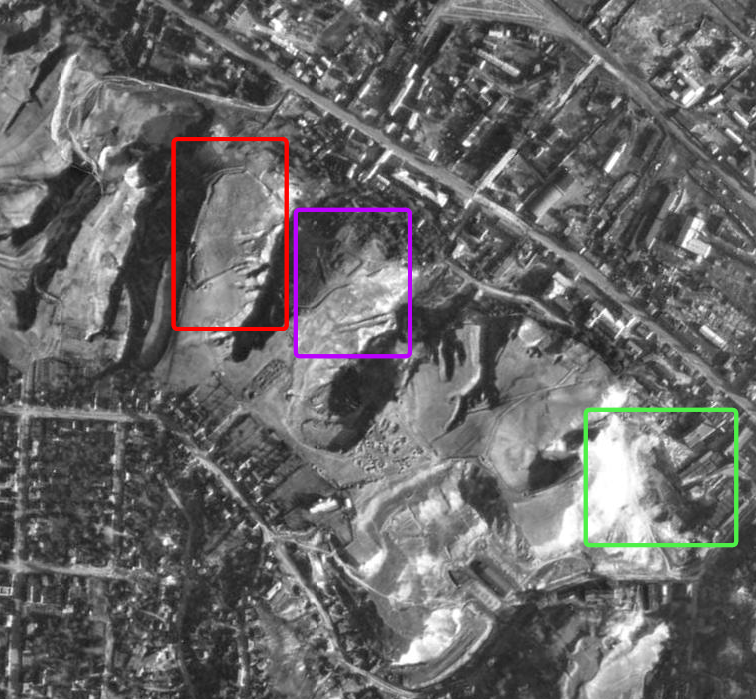
\includegraphics[width=\linewidth]{chast-kirvys/lys02/rvy-n.png}
\end{center}

На фрагменте аэрофотоснимка 1943 года их видно хорошо.

Снимок ориентирован на север. Кирпичный завод на Нижнеюрковской, 2 отмечен зеленым. Фиолетовым прямоугольником я выделил рвы и валы (особенно примечателен ромб в треугольнике). Красным – на соседнем отроге, там где теперь дачные участки «Кожевника», по периметру горы тоже видны некие следы деятельности человека, однако не буду судить, что это.

Поговорим об отмеченном фиолетовым\footnote{50°28'19.64"N 30°29'34.22"E}. В фильме «Возвращение в Логово Змиево» этот ров и вал можно узреть на видео. Что про него известно? Да так, ничего! Не это ли «замковище» Похилевича?

Петров в «Историко-топографических очерках древнего Киева» 1897 года издания сообщает:

\begin{quotation}
На Лысой горе, возвышающейся над нынешней Иорданскою церковию, доселе сохранились, по устному сообщению г. Хвойко, остатки древнего земляного вала.
\end{quotation}

Устное сообщение Хвойки... Не более. В 1947 году туда полез Каргер и в своем монументальном двухтомнике «Древний Киев» сообщил: «от городища в результате сильных оползней горы почти ничего не сохранилось». Правда, я не знаю, какую из гор осматривал Каргер – может Лысую, а может с «Кожевником».

Опишу местность по состоянию на осень 2013 года. Рельеф уже отличается от запечатленного на снимке 1943 года, но еще сохраняет примерные очертания. Вал, а вернее, естественным образом полузасыпавшийся ров между двумя валами, является юго-восточным краем вершины отрога. Вдоль рва по траве проложена тропа. Вытянутая с юго-запада на северо-восток поверхность плато изрыта ямами – небольшие дают повод думать, что здесь рылись черные археологи, а большие и прямоугольные наводят на мысль о существовании здесь некогда зданий. По карте РККА 1937 года, даже и тут были захоронения Иорданского кладбища, но по крутизне и высоте склона оврага с дорогой предположу, что такое было возможно лишь при заходе с юго-запада, со стороны Лукьяновки, а не снизу от Иорданской церкви – либо по дороге везли на самый наверх (опять же к Лукьяновке), а потом сворачивали на отрог.

Напротив него, к северо-западу через глубокий овраг со старинной дорогой на Лукьяновку, лежит другой отрог, где стоят дачные домики садового товарищества «Кожевник». 

\begin{center}
\includegraphics[width=0.88\linewidth]{chast-kirvys/lys02/\myimgprefix IMG_4367.JPG}

\textit{Вид от «замковища» на отрог «Кожевника».}
\end{center}

\begin{center}
\includegraphics[width=0.88\linewidth]{chast-kirvys/lys02/\myimgprefix  IMG_4366.JPG}

\textit{Берем чуть левее.}
\end{center}

\newpage

Овраг спускается на северо-восток к задворкам фабрики молочной кислоты (Кирилловская 53) и частично – нотной фабрики. Там, где он заканчивается, оба отрога – Лысой горы и «Кожевника» уже переходят в общий склон, идущий параллельно Кирилловской в отдалении от него на расстоянии квартальчика промзоны. Этот склон местами террасирован, видны развалины старых домов, ямы, фундаменты, сочатся родники, проложена система отвода грунтовых вод, затеяно некое строительство. К юго-восточной части оврага с дорогой к Лукьяновке примыкает, с ровными границами большая терраса, часть Лысой горы. На ней – жалкие остатки Иорданского кладбища. Спустимся туда с Лысой горы по давней тропе, идущей на углу холма.

\begin{center}
\includegraphics[width=\linewidth]{chast-kirvys/lys02/\myimgprefix IMG_2842.JPG}
\end{center}

Виднеются могильные холмики без крестов, два с крестами. На одном табличка с именем замазана белой краской, другая табличка, ржавая, многократно прострелена из пистолета. Стоит основание могильного камня с надписью: «Александра Владимировна ЗАГОРНАЯ 5/II 1916 Мир праху твоему дорогая жена и мать». 

\newpage

\begin{center}
\includegraphics[width=0.93\linewidth]{chast-kirvys/lys02/\myimgprefix IMG_4350.JPG}

\textit{2015. Уступ с остатками кладбища. Вперед пошел склон к «замковищу».}
\end{center}

\begin{center}
\includegraphics[width=0.93\linewidth]{chast-kirvys/lys02/\myimgprefix IMG_4351.JPG}

\textit{Вид в другую сторону. За треугольником уступа – овраг с дорогой, позади – бугристый склон «Кожевника».}
\end{center}

\newpage

Неподалеку, северо-западнее лежит местность Загоровщина (Загоровка) и была улица Загоровская, возможно фамилия с ними связана. В окрестностях, в 1770-х годах у Кирилловского монастыря арендовал землю по чиншу значковый товарищ Иван Загоровский, вероятно от него и Загоровщина, а может от того, что «за горой». В справочнике «Путеводитель по городу Киеву» 1911 года по адресу Мыльный переулок, 23, была усадьба некоего Загорного Г. Д. – скорее всего родич покойной.

К 2015 году появилась парочка новых безымянных крестов, а так всё осталось по-старому.

Ниже уцелевшего участка кладбища, в сторону Кирилловской, в склоне много раскопанных могил – пустые ямы. В одну такую я провалился, когда лез поглядеть, что же там отмечено воткнутым в землю металлическим дрыном. Раскопы вгрызаются и в самую кручу, способствуя оползням.

Иорданский погост – наиболее древний из сохранившихся киевских кладбищ. Только по письменным источникам его существование прослеживается с 18 века. Возможно, вид его до разрушения и забвения был подобен тихому заповеднику каменных надгробий старообрядческого кладбища на исконной Юрковице. Иорданское закрыли купно с Щекавицким, Приорским и Старо-Демиевским, постановлением Киевского горсовета в августе 1928 года.

От кладбища вниз, по направлении к Кирилловской – бывшая усадьба Марр с пивзаводом.

В конце 19 века здесь стоял «Винокуренный и дрожжевой завод Марр», принадлежащий Марии Адольфовне Марр\footnote{Не путать с купчихой третьей гильдии Христиной Семеновной Марр, которая с 1861 года владела кирпичным заводом на Сырце, кирпичи с клеймом «Х. МАРРЪ». Брат Марии Марр, Вольдемар Адольфович, держал в начале 20 века трактир на углу Жилянской и Степановской.}, а в 1909 уже купцу 2-й гильдии Иосифу Ивановичу Марру. Занимал территорию нынешних Кирилловской 53, 55, 57. При царской России имел адрес Кирилловская, 53 (теперь здесь фабрика молочной кислоты). В протяженности по Кирилловской, Иорданская церковь была между Мыльным и Иорданским переулками, а завод Марр – начинался от Иорданского переулка и до Богуславского спуска. Завод был непосредственно через переулок к северо-востоку от церковной усадьбы.

На конец 19 века можно считать, что над усадьбой Марр находится отрог с дачами «Кожевника», а над Иорданской церковью – отрог Лысой горы со рвами. 

%Таким образом усадьба Марр либо занимала часть прежней, большей чем церковная, усадьбы Иорданского монастыря (и тогда соседний Богословский был где Богуславский спуск), либо накладывается на усадьбу соседнего с ним Богословского.

В сборнике «Труды четвертого Археологического съезда в Казани» (за 1877 год, том 1, издание 1884 года) напечатан материал Антоновича, который я приведу здесь целиком за его редкостью и ценностью. Разбивка на абзацы – моя, в подлиннике таковой нет вообще. Курсив – Антоновича. Взгляды Антоновича отличны от моих – так, он предполагает Лысую гору Хоревицей, а град Киев традиционно относит к Старокиевской горе. 

Также отмечу, что в позднейшей публикации, 1895 года, «Археологической карте Киевской губернии», Антонович относит 4 языческие могилы, о коих пойдет речь ниже, к усадьбе «купца Марра». Это позволяет предположить, что речь идет о части кладбища, которая была на верху горы, где ныне дачи «Кожевника», либо у той ее части, где склон становится более пологим и террасирован.

\begin{quotation}
О ДРЕВНЕМ КЛАДБИЩЕ У ИОРДАНСКОЙ ЦЕРКВИ В КИЕВЕ (О РЕЗУЛЬТАТАХ РАСКОПОК, ПРОИЗВЕДЕННЫХ В СЕВЕРНОМ УГЛУ ГОРОДА КИЕВА)\\

В.Б. Антоновича.\\

(Читано в заседании 16 августа, См. Протоколы, стр CXIX).\\

Местность, о которой я буду говорить, известна давно в летописях г. Киева. Если обратить внимание на местные легенды, занесенные в летописи, то увидим, что город прежде не был таким, как он теперь существует, а разделялся на 3 поселка: самый Киев, Щекавица и Хоревица; к последней вероятно и относится место, где были проведены раскопки, служащие предметом моего реферата.

Оно находится в северном углу города, в нескольких верстах от центра, на равнине, ока\-ймленной с одной стороны – поемными лугами Днепра, с другой – возвышенностью. В центре этой местности существует древняя Иорданская церковь, рядом был Богословский монастырь.

Здесь в доисторическое время был центр многолюдный и торговый. Это доказывается вещами, найденными тут, – так были найдены большие клады из саманидских монет IX-X столетий, указывающих на торговлю в то время с центральной Азией. По определению этих монет оказалось, что они чеканены в Самарканде, Балке, Шаме и др. городах Туркестана и относятся к половине IX и до половины X в. 

Кроме того, несколько лет назад, разрывая один склон горы, нашли большую полость, наполненную огромным количеством костей – мужских, женских и детских, с небольшим количеством при них вещей, сваленных в большую яму; всего до 4000 черепов, – вероятно это были жертвы насильственно истребленные при разрушении этой части города.

Я указал на все это для того, чтобы характеризовать значение этой местности.

Место, о котором я буду говорить, находится в центре, где стоит Иорданская церковь. Несколько дальше к склону горы – древнее кладбище, неподалеку – развалины Богословского монастыря, потом верхняя часть состоит из уступов горной возвышенности.

Год назад, одному владельцу пришлось делать постройки в этой местности. Для этого был снят последний уступ возвышенности, причем оказались весьма интересные находки.

Часть площади покрыта была древним кладбищем, на котором в позднейшее время (в XVII ст.) выстроено было здание, впоследствии сгоревшее. При снятии земли оказался фундамент, погреба, много посуды местного изделия, относящейся к XVII ст. 

Тут же были найдены: серебряная дощечка с изображением, среди осколок посуды серебряная монета – полторак маркграфа Брандербургского Георга Вильгельма (1619-1641); так что, вероятно, здание было возведено в конце XVI или начале XVII ст.

На месте этого здания потом были могилы. За пределами его уцелели 4 могилы, представляющие каждая – особый тип погребения.

Одна из них не представляет никаких особенных характерных признаков. Но остальные три содержат характерные находки, указывающие на принадлежность могил к общеизвестным курганам железного периода, эпохи непосредственно предшествующей введению христианства.

В одной найден всадник на лошади, с полным вооружением: кольчугой, шишаком и обо\-юдо-острым мечом, характеризующим древнюю эпоху Киевского княженья. Характерно то, что голова лошади была разломлена большим камнем, найденным в черепе.

В другой могиле скелет лежит головой к западу и при нем найдено много ценных вещей, указывающих, что погребенный был человек богатый\footnote{А могилу никто не разграбил до 19 века.}.

У пояса была пряжка с медной иглой, на которую он застегивался, пряжка древне-герман\-ского происхождения\footnote{Местные мастера не могли сделать пряжку?}, точильный камень в железной оправе, у шеи скелета найдено нес\-колько сережек, состоящих из серебряных проволок, на которые надеты бусы из горного хрусталя, одни серьги без бус, другие – из золотой проволоки с бусами. Медальон, сделанный из восточной монеты, которая по определению И. Ф. Готвальда, принадлежит времени Абу-Джафар Мансура, чеканена в Куфе 142 года гиджры (полов. VIII ст.). Затем у шеи же были найдены 2 серебряные крестика, один с приделанным ушком для привески, другой снабжен гвоздями.

В 3-й могиле не было скелетов, а найдена урна из беловатой глины, содержащая жженые человеческие кости; она стояла вверх дном.

Все 3 могилы указывают на до-христианскую эпоху и судя по монете, принадлежащей к VIII в., и по типу погребения, относятся ко времени с VIII в. до принятия христианства.

Обратим внимание на две особенности найденных предметов, указывающих на эпоху более раннюю, чем княжение: 1) все вещи указывают на неумение в то время спаивать металл: концы серег, проволоки \textit{скручиваются и связываются узлом}, к монете, обращенной в медальон, приделана металлическая пластинка, \textit{приколоченная гвоздем}; затем крестик, как видно, разломанный, потом починенный: не умея спаять, вырезали из серебра пластинку, согнули ее на две половины, провели их чрез разломанное место и приколотили гвоздями.

Если сравнить с этими находками вещи, принадлежащие к эпохе княжения, то увидим, что искусство делать разные вещи из металлов было вполне известно тогда. Это ясно указывает, что найденные предметы сделаны и употреблялись в период раннего княжения.

Для доказательства можно прибегнуть к сравнительному приему.

Вот две пары серег известного типа киевских серег Десятинной церкви эпохи княжения, – таких находится бесчисленное множество на месте Киевского княжения. Характеристические признаки этого типа: более или менее толстая серебряная проволока, на которую насажены три серебряные неподвижные бусинки, иногда они делаются ажурными, но всегда есть три бусинки. Третья пара серег является прототипом первых двух, впоследствии сложившимся в излюбленный тип; в нашей находке есть серьга из серебряной проволоки, на которую насажены три подвижные бусы из горного хрусталя и композиции. 

Отсюда я делаю вывод, что мы имеем делом с кладбищем, существовавшим на ранее половины VIII ст. и не позже конца IX в. и что в то время характеристичны для степени развития местного искусства вышеприведенные черты.
\end{quotation}

Годом раньше этой публикации, в статье «Археологические находки и раскопки в Киевской губернии 1876 г.» (Чтение в историческом обществе Нестора летописца, Книга 1) Антонович сообщал подробности:

\begin{quotation}
Другая замечательная в археологическом отношении, находка относится к гораздо более позднему времени. Находка эта сделана была совершенно случайной в Плоской части Киева, в окрестностях Иорданской церкви, в усадьбе г. Марра.

Усадьба эта занимает целый квартал, ограниченный: Кирилловскою улицей, Богословским и Иорданским переулками, заднею же частью она примыкает к крутой возвышенности, на которой расположен Лукьяновский квартал и у подошвы которой, на самой закраине усадьбы г. Марра, находятся развалины какого-то древнего церковного здания (по предположению Богословского монастыря).

Значительную часть площади своей усадьбы г. Марр спланировал в этом году, для предполагавшейся постройки обширного здания. При планировки открыты были кирпичные фундаменты обширного дома, истребленного пожаром, как о том свидетельствуют обгоревшие концы бревен; дом этот, вероятно мещанский или монастырский, сгорел в XVII или XVIII столетии: в обвалившемся погребе его найдено было множество стеклянной посуды всевозможных форм и размеров и между нею одна серебряная монета – прусский шеляг с именем брандербургского курфирста Георга Вильгельма (1619-1640; затем несколько железных предметов: кирка, замок, цепи, ножик и т.п., и, наконец, в углу, посеребрянная дощечка, величиною в 1/8 листа бумаги; на доске вырезано изображение прямоугольного креста, стоящего на трех ступеньках и обвитого терновым венком [подробное описание креста]

Открытые фундаменты здания и найденные в них предметы не представляли сами по себе особенного важного интереса, но при дальнейшей планировке площади оказалось, что здание это, построенное (судя по монете) не позже первой половины XVII столетия, покрыло собою следы гораздо более отдаленной древности.

[описание четырех языческих погребений, которое Антонович дает и в статье «О древнем кладбище у Иорданской церкви в Киеве» с некоторыми подробностями – в погребении всадника были также указаны 8 наконечников стрел, два железных стремени, бронзовая с серебряной насечкой поясная пряжка, железный топор]
\end{quotation}

От погребения всадника по 1960-е в Национальном музее истории Украины сохранялся меч. На нем были клейма – испорченная надпись и узор из косых крестов. Медная проволока украшала рукоять.

Афанасий Семенович Рогович в статье «Об экскурсии, произведенной в 1875 г. по предложению Киевского общества естествоиспытателей»\footnote{ напечатанной в «Записках киевского общества естествоиспытателей» (1876, том IV, выпуск 3)} дает любопытные подробности:

\begin{quotation}
Грунт земли Кириловской улицы и вообще Подола нанеcен с гор и течением Днепра после вырытия пещер, что видно из слоев земли, обнажаемых при копании рвов под постройки, останкам животных и изделиям человека.

В том месте где находятся древние остатки монастыря Иоанна Богослова, недалеко Иорданской церкви в усадьбе Марра, при копании рва, на глубине более двух саженей в желтой глине обнажился слой раковин, тех же самых видов, которые и в настоящее время водятся в Днепре;

в верхнем черноземном слое толщиною до полутора сажени, в нижней его части найдена печь для сожигания покойников, горшки с посмертным пеплом и уцелевшими полуобгоревшими костями человеческими, серьги из серебряной проволоки с надетыми на нее одною или тремя разноцветными бусами, одна сережка из золотой проволоки, серебряная куфическая монета с приделанным ушком для ношения на шее; 

над языческим кладбищем, на незначительной глубине находятся остатки татарского побоища: множество черепов татарских и славянских перемешаны между собою и похоронены без всякого порядка\footnote{Не об этом ли месте говорил Антонович касательно останков 4000 человек?}; 

в одной из могил найдено три скелета человеческих вместе с скелетом лошади, седло с стременами.

Голова всадника и лошади раздроблены кистенем, круглым булыжником, зашитым в кожу, найденным вблизи скелетов; в той же яме найдены большой железный меч, копье, верхняя часть железного шлема, имеющая вид чашки, два тонких серебряных креста, сумка с железными стрелами, небольшой брусок, вероятно, употреблявшийся для точения стрел, часть пояса и две больших вызолоченных медных пряжки с выпуклыми украшениями, из которых наибольшее имеет вид великокняжеской шапки, игла из красной меди и железный бердыш.
\end{quotation}
 
Получается, всадника и лошадь подвели к могиле, убили здесь же на месте и с почетом погребли. Ритуальное убийство?

В «Археологической карте» Антонович приводит сведения о более ранней находке, монетном кладе:

\begin{quotation}
Иорданская церковь. В 1863 году на церковном погосте найден клад, состоявший из 192 серебряных саманидских диргеммов 895-930 годов, также 2 серебряные перстня, серебренные: цепочка и привеска. Музей Киевского университета. Беляшевский 21.
\end{quotation}

По книге Каргера я отыскал некоторые подробности этого:

\begin{quotation}
В 1863 г. в Подольской части Киева, на кладбище Иорданской церкви, на глубине около 1,5 м. был найден еще один клад, состоявший из ста девяноста двух серебряных куфических монет, двух серебряных пластинчатых перстней с завязанными концами, круглой серебряной подвески, покрытой зернью, и небольшого куска серебряной проволоки. Клад находился в глиняном сосуде, разбитом в мелкие куски при обнаружении клада.

За исключением одного диргема (911-912 гг.), поступившего в Эрмитаж, Иорданский клад был целиком приобретен Минц-кабинетом Киевского университета, откуда позже был передан в Киевский исторический музей, где находится и поныне.

Монетная часть клада, по определению Лерха, состоит из одного тагеридского диргема, чеканенного в Фарсе в 232 (905-906) г., и ста семидесяти восьми саманидских диргемов, битых в Шаше, Самарканде, Нисабуре, Балхе, Андерабе, Педжхире и Мерве в 895-936 гг.

В кладе находилось, кроме того, двенадцать подражаний саманидским диргемам Насра, сына Ахмеда, чеканенным с Самарканде.

Клад был зарыт в землю, очевидно, не ранее середины X в.

Девять монет Иорданского клада (904-925 гг.) имеют пробитые отверстия, а в двух случаях, кроме того, припаянные ушки для подвешивания. По-видимому, вместе с упомянутой выше круглой подвеской, украшенной зернью, эти монеты составляли некогда ожерелье. Возможно, что подвеска и монеты были нанизаны на тот кусок тонкой серебряной перегнутой проволоки, которая была найдена в том же кладе.

Серебряная тисненая, покрытая зернью круглая подвеска и пластинчатые с гравировкой серебряные перстни могут быть отнесены к началу X в., т.е., по-видимому, современные поздним монетам клада.

В 1878 году на Подоле в усадьбе Марра, известной благодаря найденному там погребению X в., была найдена аббасидская монета, битая в Куфе в 142 (759) г., отделанная в виде медальона для ношения в составе ожерелья. Весьма вероятно, что монета происходит не из клада, а из погребения.
\end{quotation}

Находки восточных монет тем более примечательны, что в былинах цепь холмов Кирилловских высот именуется Сорочинскими горами. Сорочины – то же, что «сарацины». Так называли восточных людей, арабов, мусульман. Учтем также, что наверху этих холмов лежит бывшая часть Лукьяновки – местность Татарка, где жили Татары. Возможно, во время, к которому относятся монеты, «сарацины» играли в районе Лысой горы и окрестностей одну из главных ролей.

Наступило время поговорить и о деятельности в этой местности Кондрата Андреевича Лохвицкого (1774/75 – 1849). В ученой среде над ним принято посмеиваться, признавая, однако, важность сделанных им некоторых открытий – остатки Золотых ворот, фундамент Десятинной церкви, а также руины, в коих предполагают Ирининскую церковь. Многие итоги раскопок Лохвицкого и сделанные им, подчас под влиянием покровителей, выводы, считаются спорными. 

Можно долго об этом рассказывать, как и о самом Лохвицком. Он со своими мистическими исканиями, снами-пророчествами\footnote{С записками Лохвицкого за 1798, и 1808-1819 годы работал Ф. Терновский и цитировал их в «Материалы для истории мистицизма в России (Записки К. А. Лохвицкого)» – см. Труды Киевской Духовной Академии. 1863. Т. 3. В архивах сохранились и более поздние записи, время от времени всплывающие в публикациях. Вот пример за 19 декабря 1831: «Сегодни видел во сне явственно: по утру в 7 часу. Слово слышал говорящее в душе моей: «Сделай себе Крест ┼ в воображении. Исповедуйся пред ним». (Проснулся) Я проснувшись пел в душе моей: «Кресту Твоему поклоняюся Владыко, и Святое Воскресение Твое пою и славлю». (Был исполнен радости духовной)».}, раскопками и прочими деяниями заслуживает отдельной книги. Глава же о другом.

Впрочем скажу, иногда трактовки находок появлялись следующим образом. Например, Лохвицкий раскапывал на Андреевском спуске. Нашел кроме прочего кнут, «что волов погоняют», повез его к генерал-фельдмаршалу Остен-Сакену, своему патрону. Тот берет кнут в руки и говорит: «Сегодня празднует церковь российская в Киеве Святому князю Владимиру, то это его кнут открылся. И что оставил на память: как всех тогда не переучил, то чтоб теперь доучить киевлян». И приказал Лохвицкому беречь кнут.

В районе Иорданской церкви Лохвицкий тоже занимался раскопками, и не без успеха. Его находку позднейшие ученые трактовали как остатки Иорданской церкви святого Николая, и связывали с ней, а не с Николой Добрым, «чудо о пленном половчанине». Насколько я понимаю, эти историки подозревали в руинах церковь, которую разбирал и ломал Войтех Соколовский.

Что же и где нашел Лохвицкий? Что он сам думал по этому поводу? В 19 веке Николай Оглоблин среди бумаг своего покойного отца, ключаря Киево-Софийского собора протоиерея Н. Я. Оглоблина, наткнулся на записки Лохвицкого. И снабдив их вводной статьей, опубликовал в 26 нумере «Киевской старины» (июль 1889 года) под заглавием «Из бумаг Лохвицкого».

Привожу записку, касающуюся развалин близ Иорданской церкви, целиком, ибо в ней излагается не только суть находки, но и доводы в пользу того, что это именно древняя Ильинская церковь, которую прочие ученые полагают ныне на Подоле на стыке Ильинской и Почайнинской улиц. Речь идет о летописной церкви Ильи «над ручаем», к которой «водили роте» варягов при Игоре.

\begin{quotation}
Записка о раскрытии места древностей варяго-российской церкви Ильинской.\\

Чиновник 5 класса Лохвицкий, соревнователь Московского общества истории и древностей российских, руководствуясь собственным поручением г-на фельдмаршала графа Сакена и письменным предписанием военного киевского, волынского и подольского генерал-губернатора графа Левашова, в сходствие Высочайших повелений 29 июля 1824 г. и 4 генваря 1833 г., нашел место фундаменты каменные (было написано и зачеркнуто: «начал раскапывать с 5 мая сего 1832 года древность первой в России церкви Ильинской», прим. Оглоблина) церкви Ильинской варяго-россов, времени великого князя Игоря.

Сия церковь до сего времени была известна только по истории, местопребывание же ее совсем утеряно у историографов, даже неизвестно было – из какого материала она построена. Следовательно, история не имеет сведений и о плане сей церкви.

Преподобный Нестор об ней пишет (в летописи по Кенигзбергову списку, изданному в С.-Петербурге в 1776 г., на стр. 44 и 45): в 945 г. «Христианскую Русь водиша роте (к присяге) в церкве святаго Ильи, яже есть \textit{над ручьем}, конец Постничи (sic) беседы, в Козарех: се бо бе соборная церковь, мнози бо беша \textit{варяги} хрестьяне». Сие свидетельствуется при договоре великаго князя Игоря с греческим императором Романом...

Но поелику Нестор утверждает о христианах сей церкви, что они были варяги, а варяги, или скандинавы, или шведы были католической веры, из сего заключить следует, что сия церковь была католическая, ибо при Игоре не было разделения (?!! – прим. Оглоблина) настоящего вероисповедания \textit{католического} с греческим у варяго-россов, но по принятии россиянами греческой веры при великом князе Владимире в 988 г. отделились греко-российской веры христиане от католиков. По сей причине Ильинская церковь до сего времени \textit{от старожилов киевских} называется «костелом», а костел есть римско-католического вероисповедания.

Место сей церкви и остатки фундаментов каменных, отрытых из недр земли при изследовании Лохвицким, находится на выезде из Киева в Кирилловское богоугодное заведение, за Иорданскою церковью, от дороги по левой стороне, повыше бывшей Богословской церкви, в полгоры над ручьем так называемым Иорданским.

Ручей Иорданский пониже и подле сего места течет, а вытекает повыше, с горы, близ сих остатков Ильинской церкви. Сей ручей начало берет из ключей железистых, которые приметны по ржавчине железной в источнике родника сих ключей. Вода сего ручья чистая, свежая, и по испытанию полезна для здоровья. Ручей впадает в озеро называемое Иорданское, находящееся на Оболони. Из сего озера Иорданского вытекает речка Почайна и упадает в реку Днепр.

Строение каменных фундаментов сей Ильинской церкви доказывает самое древнейшее происхождение ее: в фундаменты положены огромные нетесаные камни, между кирпичами древней работы, тонкими, шириной в шесть, а длиною в восемь вершков, на цемент, который так связал дикие камни с кирпичом, что трудно ломом отделить. В кирпиче масса так крепка, как крепкий камень. В цементе и в кирпичах приметен толченый кирпич, алебастр и уголь. – По разрытии земли и обнаружению фундаментов между щебнем довольно оказывается росписного по щекатурке красками, которые можно еще различать...

Церковь сия должна быть обширная, судя по положению пространного бугра, покрытого землею более сажени. Но как все здание требует большего разрытия и на то значительных издержек, будучи в полгоры заплыло землею глинистою с гор, то и остается еще не совсем раскрытое, а потом и плана снять нельзя. 

Следовательно, требуется дальнейшее изследование и подтверждение достовернейшее о точности сего места, Ильинской церкви принадлежащего, ибо по сим обстоятельствам (т.е. вследствии недостаточного исследования развалин автором..., прим. Оглоблина) и митрополит киевский и галицкий (Евгений Болховитнов, прим. Оглоблина), осматривающий сие раскрытие 4 июля усумнился в существовании когда либо в сем месте Ильинской церкви. – Корреспондент Общества Московского истории и древностей, чиновник 5-го класса Кондрат Лохвицкий.

Примечание Оглоблина: внизу «Записки» стояла сначала дата: «августа 26 дня, 1832 года», затем зачеркнута и написана новая: «июля 15 дня, 1834 г.». Несомненно отсюда, что «Записка» составлена в 1832 г., а в 1834 г вновь пересмотрена и исправлена Лохвицким собственноручно.
\end{quotation}

Я к этому ничего не прибавлю, оставив вам самим рассуждать над сказанным.

В 1899 году, Николай Федорович Беляшевский раскапывал на Лысой горе, давней Юрковице, курганы и многое другое. Наибольший из курганов получил название Кургана-Могикана.

\begin{center}
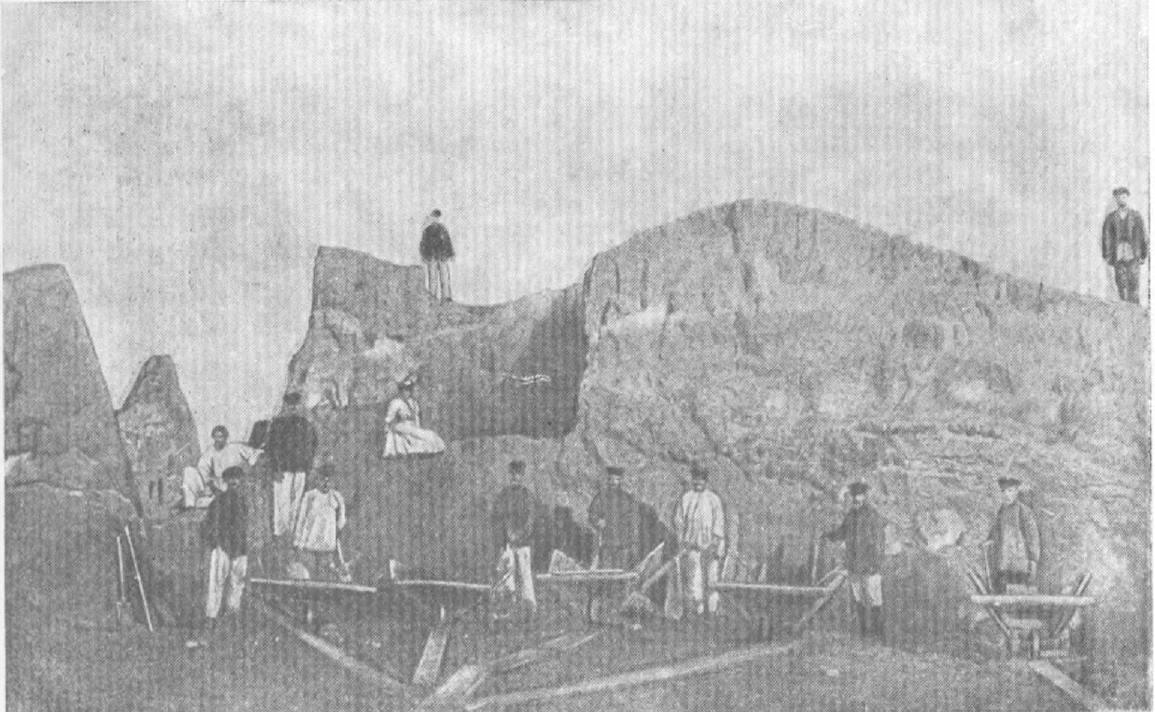
\includegraphics[width=\linewidth]{chast-kirvys/lys02/1899-mogikan.jpg}

\textit{Раскопки кургана Могикана, 1899.}
\end{center} 

Сведения об этом разбросаны по трем источникам. Статьи Скрыленко и Беляшевского в АЛЮР (Археологическая летопись Южной России), которые мне недоступны. Пересказ оных у Каргера. И в 6 томе «Киевской старины» за 1899 год я отыскал «беглый отчет» о раскопках Беляшевского. Эту статью и приведу ниже со своими примечаниями.

%у Каргера положение описывается так:

%\begin{quotation}

%на Верхней Юрковице, в усадьбе Лурье и Левина, при планировке местности в связи с постройкой кирпичного завода. На возвышенной части упомянутой усадьбы, отделенной оврагом от соседней усадьбы Иорданской церкви, до 1899 года, сохранился большой курган [...]
%\end{quotation}

%Хоть бы указание было, в какую сторону отделенный оврагом... В справочнике 1882 года указана усадьба купца Соломона Лурье на улице Нижняя Юрковица, 37 – эдак за десяток домов от дома поручика Чеберяка.

\begin{quotation}
Раскопки на Верхней Юрковице\footnote{Где-то на «Верхней Юрковице» проводил раскопки могил и Турвонт Венедиктович Кибальчич (1848-1913), о чем есть сведения во втором томе протоколов «Антропологической выставки», изданных в 1878 году – источник я не читал, знаю по упоминанию у Каргера. Кибальчич выставил четыре черепа с раскопок на всеобщее обозрение.} в г. Киеве.

Нагорная площадь, занятая Верхней Юрковицей, разделена со стороны Кирилловской улицы несколькими оврагами очень давнего происхождения, образованными стоком атмосферных и подпочвенных вод; на плане этот край площади имеет вид нескольких мысов, вдающихся в долину Днепра.

Один из таких мысов, разделенный оврагом от другого, на котором расположено кладбище Иорданской церкви, и был местом раскопок. 

На этом месте с весны начаты работы по устройству кирпичного завода (Лурье и Левина)\footnote{В справочнике 1882 года указана усадьба купца Соломона Лурье на улице Нижняя Юрковица, 37 – эдак за десяток домов от дома поручика Чеберяка. В деле Бейлиса упомянута еще «маслобойня Лурье». Ничего более этого про Лурье сообщить не могу.}; в конце апреля приступлено было к спланировке площади и уже при начале работ обнаружены некоторые признаки, указывающие на то, что местность эта представляет интерес в археологическом отношении.

На них было обращено внимание живущей по близости госпожой Скриленко\footnote{Археолог Антонина Антоновна Скрыленко. В Киеве была сотрудницей Киевского музея древностей и искусств, а также помощницей и секретаршей Викентия Хвойки. Большинство черновиков его писем написаны рукой Скриленко. В переписке Хвойки с английским археологом Ellis Hovell Minns последний постоянно передает Скрыленко приветы и поклоны – они были знакомы лично. Предположу, что Скрыленко играла в научных исследованиях большую роль, однако по некой причине оставалась в тени Хвойки. Вообще при чтении переписки с Миннзом мне показалось, будто письма от Хвойки сочиняли двое – Скрыленко и Хвойка, а иногда даже одна Скрыленко. Скрыленко проживала на Кирилловских высотах (адрес за 1900 год: Киев, Верхо-Юрковская улица, дом 8 – собственный дом), а Хвойка тоже имел дом неподалеку, только внизу под Кирилловскими высотами. Будучи в Киеве, Скрыленко переводила с чешского «Slovanske Starozitnosti» доктора Любора Нидерле (L. Niederle), принимала участие в раскопках, в том числе с Беляшевским. В 1905 по приглашению Дмитрия Яворницкого перебралась с сыном в Екатеринослав (Днепропетровск), чтобы работать заведующей («хранителем») местного Екатеринославского областного музея им. А. Н. Поля. Однако рабочие отношения с директором музея Яворницким стали враждебными, и Скрыленко в 1906-м вынуждена была оставить должность. В 1908 году Антонина Антоновна уже преподавала, в том же Екатеринослав, иностранные языки в женской гимназии. По некоторым данным, позже Скрыленко покинула этот город.}, интересующейся местными древностями, – не будь этого обстоятельства, очень возможно, что и эта местность, как и многие другие в черте Киева, осталась бы не обследованной в научном отношении. А. А. Скриленко любезно поделилась с нами своими наблюдениями и в течении всего истекшего мая принимала участие в раскопках, ближайшее наблюдение над которыми взял на себя составитель настоящей «Летописи».

Мыс, о котором мы говорим, занимает площадь приблизительно в сто квадратных метров; на северо-восточном краю его находятся 3 кургана – одни из последних, уцелевших на территории Киева\footnote{Северо-восточный край – вероятно, речь идет о части Лысой горы, примыкавшей с юга и юго-востока к Мыльному переулку. Современный Мыльный переулок уходит во глубину оврага, носящем явные следы добычи глины. На плане первой половины 19 века там просто большой овраг, а на аэрофотоснимке 1943 – уже чудовищное и широкое глинище.}.

Съемка земли производилась на всем пространстве этого мыса, съемка шла глубоко, захватила собой не только поверхностный слой чернозема но и довольно большой слой материка; приходилось только внимательно следить за работами, в нужных случаях приостанавливать их и сами исследовать тот или другой пункт.

Раскопки показали, что весь этот мыс был заселен в неолитическую эпоху каменного века. Следы первобытной жизни сосредотачивались главным образом по краям мыса; здесь в нескольких местах обнаружены т. н. сорные кучи, имевшие вид углублений и ям, наполненных речными раковинами, костями различных животных и рыб, углями и черепками от сосудов ручной лепки.

На северо-западном откосе встретились также остатки очага, состоявшие из пережженной глины; другой очаг, с массой лежавших возле него костей животных, открыт в центральной части мыса.

Собранная здесь коллекция этой эпохи является довольно разнообразной и полной. Мы имеем тут несколько представителей каменных орудий: кремневый топорик – клин со шлифованным лезвием, кремневое острие со вторичной подправкой, части отбивных ножиков; несколько изделий из рога и кости: 2 роговых топорика, костяное долотцо и шило.

Особенно же богат отдел керамики: кроме нескольких небольших сосудов, добытых в более или менее целом виде, коллекция заключает в себе несколько сот черепков от сосудов разной величины, формы и толщины стенок, без орнамента и покрытых разнообразным орнаментом из углублений, шишек, нарезов, бороздок и т.д.; у многих из черепков сохранились ушки, у более тонких из них обжиг прошел насквозь, более же толстые имеют в средине плохо обожженную прослойку.

Что сосуды служили для приготовления пищи, то на это указывает найденная часть одного сосуда, на дне которого сохранился слой рыбьих костей\footnote{Не вижу в том, что в части одном сосуде были рыбьи кости, указания на приготовление в сосуде пищи и на сходное предназначение других найденных сосудов. В будущем найдут кусок мусорного бака с прилипшей жвачкой, и следуя этой же логике, решат, что в мусорном баке готовили жвачку.}.

Из других глиняных предметов найдено нес\-колько пряслиц, пока еще не объясненные предметы в виде четырехугольных с вытянутыми углами пластинок с утолщением посредине и часть грубо вылепленной человеческой фигурки.

Культура, открытая в данной местности, не представляет из себя ничего нового: подобного же рода находки были сделаны в других местах, по той же нагорной стороне Кирилловской улицы; впервые она обнаружена в 1876 году профессором Антоновичем, исследовавшим здесь пещеры в лессе, относящиеся к тому же времени.

Последующие недавние раскопки г. Хвойки дали новый обильный материал, так что наши находки прибавляют к нему сравнительно немного, и только следует пожелать, чтобы добытые раньше данные были обработаны и стали полным достоянием науки, пока же оне известны лишь по отрывочным сведениям.

Из трех, находящихся здесь, курганов вполне раскопан пока лишь один – самый больший, расположенный ближе всего к краю мыса\footnote{Он-то по другим источникам и проходит как Курган-Могикан.}.

Окружность его у основания – более 40 метров, высота же около 2-х метров. В первоначальном виде курган был несомненно выше, испортили его кладоискательские раскопки, от которых остались следы в виде довольно глубокого колодца в вершине кургана.

Исследование этого кургана дало следующие результаты.

Под насыпью оказалась четырехугольная могильная яма, длиной по направлению с севе\-ро-востока на юго-запад 4,5 метра, шириной 3 метра 15 стм., ко дну ямы, лежавшего приблизительно на 1,5 м. ниже горизонта, бока ея немного суживались; яма выкопана в желтой глине, дно же ея составлял следующий под желтой слой белой, очень твердой глины. 

Нетронутой оказалась юго-западная часть могилы; здесь, почти у самой стенки ямы, лежал в вытянутом положении скелет человека, головой на юго-восток; при верхней части скелета не оказалось почти никаких предметов, если не считать найденного в области груди плоского камушка – голыша, жилки которого, перекрещиваясь, образуют как бы крест, присутствие его скорее всего можно считать случайным.

У левой руки скелета найдены 3 стеклянные бусы, из которых две из разноцветной стеклянной массы, и бронзовая круглая пуговка.

Большинство же находок сосредотачивалось у нижних конечностей: у ступни правой ноги лежала железная шпора, состоящая из дужки с острым стержнем у вершины, бронзовое литое кольцо и части какого-то железного предмета, почти совсем уничтоженного ржавчиной. Под правой ступней, почти совсем на белой глине, найден предмет из распиленной вдоль широкой части лосьего рога, 19,5 стм. длиной, с выемкой с одной стороны, украшенный резной звериной головой и снабженный сквозными дырочками – быть может часть налучья; рядом с этим предметом лежали кости какого-то мелкого животного.

Между нижними частями ног найдена железная пряжка, здесь же стоял деревянный точеный сосуд в виде чашки, совершенно конечно истлевший, сохранилась лишь в нетронутом виде серебряная оковка чаши, состоявшая из тонкой полоски серебра, прикрепленной к чаше серебянными же гвоздиками; у чаши повидимому была и ручка, т.к. и для нее имеется широкая, частою вызолоченная, оковка; кроме того, тут же находились 3 небольшие четыреугольные серебрянныя пластинки с гвоздиками для прикрепления, из них одна прирезная; диаметр верхней части чаши – 14 стм.

Как скелет, так и все найденные возле него предметы добыты из твердой, плотно слежавшейся земли. Характер почвы остальной части могильной ямы был иной – сюда повидимому проникли кладоискатели, земля здесь рыхлая и содержимое ямы представляет полный беспорядок.

На разной глубине тут найдены остатки повидимому трех скелетов; кроме костей, встретились и некоторые предметы: в северном углу ямы, под находившимся здесь черепом, лежала железная шпора, подобная предыдущей, и возле нее железный окислившийся предмет, быть может подковка от сапога; в этой же части ямы, найдена бронзовая прорезная ручка от кресала, в виде двух птиц, соединивших клювы над помещенной в середине человеческой фигуркой; в центральной части могилы, на самом дне, найдена маленькая слезничка из зеленого стекла – благодаря плотности почвы и тонкости сосудика, его не удалось добыть в целом виде.
\end{quotation}
\vspace*{\fill}
\begin{center}
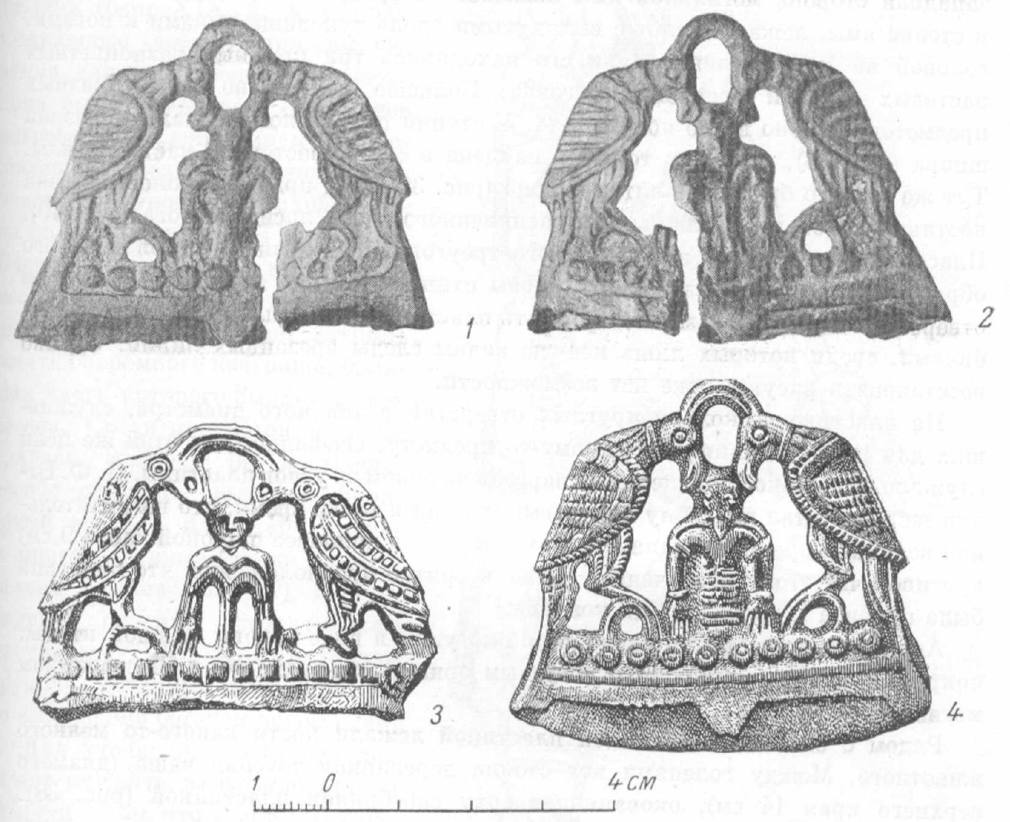
\includegraphics[width=\linewidth]{chast-kirvys/lys02/1899-mogikan-kresalo.jpg}

\textit{Найденная под Могиканом рукоять кресала (рис. 1, 2 и – подобные ему из Прикамья – 3, 4).}
\end{center} 
\vspace*{\fill}
\newpage

Статья продолжает:

\begin{quotation}
Таково содержание кургана. Характер предметов и отчасти способ погребения указывают на славянскую языческую эпоху, так что могилу эту можно отнесть к IX-X веку. Очень интересными представляются некоторые детали погребального ритуала, служащие дополнением как к письменным, так и археологическим данным по этому вопросу, в частности, раскопки этого кургана приносят свою долю в историю древнего Киева.

Раскопки остальных двух курганов еще не закончены, но, судя по некоторым признакам, они не обещают того, что дал первый курган, и даже могут оказаться не могильными насыпями, так как, не смотря на произведенную уже сравнительно большую съемку земли, признаков могильных ям пока не обнаружено.

С юго-западной стороны курганов встречено 3 погребения без наружных признаков, но относящихся к той же эпохе, что и курган.

Скелеты помещались в ямах, глубиной 1-1,5 метра, головой на запад, с вытянутыми ногами и с руками, скрещенными на груди; погребения здесь совершались в гробах, так как при каждом из скелетов найдены железные гвозди и порошок от истлевших досок гроба; находки предметов незначительны: на правой руке одного скелета находилось серебряное кольцо, украшенное чернью, у другого на руке найдено подобное же кольцо, а у головы стеклянная и серебряная бусинки, у третьего костяка возле правой ноги стоял небольшой сосуд с волнообразным орнаментом; погребения такого рода встречались и раньше по близлежащим возвышенностям.

В заключение упомянем еще о целом ряде открытых здесь же могил, в некоторых случаях снабженных склепами из кирпича-сырца; по сохранности могил, характеру кирпича и некоторым находкам, их можно отнести к новейшему времени – к XVII-XVIII векам.

Ограничимся пока этим беглым отчетом, который будет еще дополнен по окончании раскопок.

Предметы, добытые раскопками, требуют еще более детального изучения и определения (как например масса костей животных из сорных куч каменного века); предназначены они для будущего киевского музея.
\end{quotation}

%Я нашел в справочниках усадьбу некоего Соломона Лурье на Юрковской улице, но то угол Юрковской и Туровской, внизу ближе к Гавани – не подходит. А на Верхней Юрковице, на улице Половецкой, жил Корье, может его спустали с Лурье, не знаю. В адресной книге 1882 года в строке «Карсе (б. Кибальчича) 11», фамилия Карсе перечеркнута, снизу приписано «Лурье», затем Лурье перечеркнуто и выше Карсе поставлено «Корье». Однако в деле Бейлиса за 1911 год упомянут маслобойный завод некоего Лурье, возможно на Юрковице. 

Из книги Каргера можно узнать небольшие дополнения к описанию раскопок Могикана – что могильная камеры была кубической, а сверху перекрыта досками, и уже поверх них насыпан курган.

В этой главе я собрал сведения об основных находках на Лысой горе (нынешней Юрковице) близ исконной Юрковицы. А сколько их пропало за века уничтожения склонов? Как назло, земля, обжитая гораздо раньше, чем «Старый город», изувечена, исследована плохо, отрывочно, и пожалуй, дальше будет только хуже. Вместо создания тут заповедника – промышленные объекты, стройки, автобазы. С юга на уцелевший отрог наползает застройка.

Как и почему языческий, окруженный курганами град Киев на Лысой горе перестал существовать, и когда отхлынула от него жизнь, мы уже не узнаем. Резко ли всё переменилось или постепенно пустело обжитое место? Может, о первом соображении свидетельствуют найденные Антоновичем тысячи останков. Отчего же на удобные, защищенные от неприятеля и половодья высоты не вернулись люди?

Кроме выгодного расположения, обжитость в древности Кирилловских высот и Оболони имеет и другие причины. Это гончарство, коего мы коснемся позже, и металлургия.
